\documentclass[german]{book}
%\usepackage{url}
\PassOptionsToPackage{hyphens}{url}\usepackage[breaklinks=true]{hyperref}
\usepackage{dsfont}
\usepackage{listings}
\usepackage{german}
\usepackage[utf8]{inputenc}
\usepackage[final]{graphicx}

\begin{document}

\title{Open Historical Data Map\\
Systembeschreibung \\
Version 0.0.0
}

\author{
Thomas Schwotzer \\
Mohamadbehzad Karimi Ahmadabadi\\
Daniel Schulz\\
nächste/r Projektleiter/in\\
(Herausgeber)
}

\maketitle

\tableofcontents

\chapter{Überblick}
\section{Dokumentengeschichte}
\begin{table}[h]
 \begin{tabular}{|l|l|p{4cm}|}
 \hline
 Zeitraum & PL/Autor(en) & Änderungen \\
 \hline
 Wintersemester 2017/18 & Thomas Schwotzer & 
 Initialer Text
 
  \\
 \hline
 Wintersemester 1980/81 & IHR NAME & 
text \newline 
text \newline 
 
  \\
 \hline
 
 
 \end{tabular}
 \caption{Dokumentengeschichte}
 \end{table}

\section{Ziel des Systems}
Open Historical Data Map (OHDM) versteht sich als offene und freie Plattform zur Speicherung, 
Abfrage und Visualisierung orts- und zeitgebundener Daten.

Primär sind damit {\bf Karten} gemeint. OHDM erlaubt die Speicherung von Vektorgeometrien
und generiert basierend darauf Karten, die über einen Web-Map-Service (WMS) angeboten werden,
siehe Kapitel \ref{wms_wfs}.

Das zentrales Konzept aber von OHDM ist das {\bf historische Geoobjekt}. Ein Geoobjekt
ist ein menschliches Artefakt, das zu einem oder mehrere Zeitpunkten einem Raum auf der
Erdoberfläche zugeordnet werden kann. 

Zum Management der Geometrien und der Geoobjekte entstehen eigene Editoren für OHDM.

Geoobjekten lassen sich weitere Daten zuordnen, vor allem Bilder, aber auch Sensordaten. 

OHDM Nutzer sollen historische Daten in das System laden können und diese dann per WMS 
anschauen können. OHDM wird eine Linked Data Schnittstelle anbieten und wir arbeiten an einem
SPARQL Endpoint.

\subsection{Historische Karten}
OHDM-Geoobjekte sind damit alle Gebäude, Straßen etc. die von Menschen geschaffen wurde.
Aber auch Verwaltungsgrenzen jeder Art sind Geoobjekte, ebenso wie Ereignisse, die sich 
Orten zuordnen lassen (Schlachten, Versammlungen, Revolutionen etc. pp.)

In jedem Fall können damit Geoobjekten Geometrie zugewiesen werden. Diese Zuordnung ist
in jedem Fall abhängig von der Zeit. Möge unsere Hochschule, die HTW Berlin, als Beispiel
dienen. Im Jahr 2017 hat die HTW mehrere Standorte in Berlin und auf jedem Standort existieren
mehrere Gebäude und Wege. Man kann daher ein Zuordnung. Es gibt eine Reihe von Geometrien,
die die Gebäude und Wege beschreiben. Man kann diese nun dem Objekt HTW zuweisen. Diese 
Zuweisung gilt aber für das Jahr 2017.

Vor einige Jahren entstand ein zusätzlicher Campus in Oberschöneweide, dafür wurden andere
Standorte abgegeben. Die Grundrisse der Gebäude haben sich nicht geändert. Die Zuordnung
der Geometrien zu den Geoobjekten haben sich aber geändert. 

Manche Geoobjekte änderten aber auch im Laufe der Zeit ihre Position 
(wie die Siegessäule in Berlin oder der Obelisk auf dem Place de la Concorde in Paris).
Viele Gebäude beherbergen über Jahre hinweg ganz unterschiedliche Objekte. Das aktuelle
Finanzministerium der Bundesregierung ist im Jahre 2017 im gleichen Gebäude in dem zuvor die
Treuhandanstalt war.

Anhand dieser Daten lassen sich historische Karten erzeugen. OHDM bietet eine WMS und WFS
Schnittstelle an, über die historische Karten angezeigt werden können, siehe auch http://ohdm.net

\subsection{Historische Daten}
OHDM erlaubt die Speicherung von Daten mit einem zeitlichen und örtlichen Bezug.
Aktuell arbeiten wir an der Integration von Sensordaten und von Daten, die einem Geoobjekt
zugeordnet werden können.

\subsubsection{Sensordaten}
Einige Arbeiten beschäftigen sich derzeit an Daten wie Temperatur, Feinstaubkonzentration, Luftfeuchtigkeit 
und Luftdruck. Sensordaten sind zeitliche und örtliche Größen. Messungen sind in der Regel 
punktuelle Messungen. Derzeit wird an Schnittstellen für den Import von Sensordaten in OHDM gearbeitet.
Die Visualisierung der Daten wird auch hier mittels WMS angeboten werden.

\subsubsection{Daten für historische Objekte}
Aktuell wird bei Geoobjekten vor allem an menschliche Infrastruktur gedacht (Häuser, Straßen etc.).
Administrative Objekte (Länder, Verwaltungsbezirke etc.) kommen hinzu.

Wir viele solcher Objekte lassen sich historische Dokumente (Bilder, Verweise auf Webseiten) finden.
Das können Bilder sein, aber auch Urkunden. Es können aber vor allem auch alte Karten sein.

Alte Karten sind in OHDM dann nutzbar, wenn sie gescannt vorliegen. Diese Rasterdaten können
Geoobjekten zugewiesen werden. Alte Karten können aber auch Basis für die Editoren sein, siehe 
Abschnitt \ref{editoren}.

Derzeit wird an einer Schnittstelle gearbeitet, die den Import solcher historischer Daten 
in OHDM erlaubt. Die Visualisierung wird als weiterer WMS-Layer in OHDM erfolgen.

\subsection{Importschnittstellen}
Derzeit wird an folgenden Importschnittstellen gearbeitet:

\begin{itemize}
\item
Import von GeoJSON
\item
Import von RDF-Files

\end{itemize}

\subsection{Anfrageschnittstellen}
Derzeit wird an folgenden Anfrageschnittstellen gearbeitet:

\begin{itemize}
\item
Linked Open Data Schnittstelle: Geoobjekte werden über URI referenzierbar.
\item
SPARQL-Endpoint
\item
GeoSPARQL-Endpoint
\item
Integration von CIDOC-CRM
\end{itemize}



\chapter{OHDM-Datenmodell}
\section{Dokumentengeschichte}
\begin{table}[h]
 \begin{tabular}{|l|l|p{4cm}|}
 \hline
 Zeitraum & PL/Autor(en) & Änderungen \\
 \hline
 Sommersemester 1980 & IHR NAME & 
text \newline 
text \newline 
text \newline 
text \newline 
text \newline 
text \newline 
 
  \\
 \hline
 Wintersemester 2017/18 & Behzad Karimi & 
Bild eingefügt (Bilder ab jetzt mit 120mm einfügen) \newline 
text \newline 
text \newline 
text \newline 
text \newline 
text \newline 
 
  \\
 \hline
 \end{tabular}
 \caption{Dokumentengeschichte}
 \end{table}

\section{Aufgabe der Komponente}
<<<<<<< Updated upstream
%\begin{figure}[h!]
%\centering
%\includegraphics[width=127mm]{ohdm_datenmodell/ohdm_data_modell.png}
%\caption{OHDM Datamodell}

%\label{fig:datamodell}
%\end{figure}


=======
\begin{figure}[h!]
\centering
\includegraphics[width=127mm]{ohdm_datenmodell/Bilder/ohdm_data_modell.png}
\caption{OHDM Datamodell}
\label{fig:datamodell}
\end{figure}
>>>>>>> Stashed changes
Im Datenmodell von OHDM geht alles vom Geoobjekt (geoobject) aus. Dieses zentrale Object beschreibt alle Modelle auf der Karte, da alle Informationen der Modelle auf das geobject verweisen. Das einzige Objekt worauf das geobject verweist, ist der Ersteller (external\_users). Der Ersteller des Objekts greift durch ein externes System (external\_systems) auf dern Server zu und gibt die Informationen über das Geobjekt weiter. Wie nun ein Geobjekt im Allgemeinen aussieht wird im nächsten Abschnitt beschrieben.

\subsection{Geometrien in GIS}
Da OHDM mit PostGIS arbeitet (für GIS siehe ...) werden die zweidimensionalen Objekte als Polygone repräsentiert. Polygone bestehen dabei aus Punkten (points) und Linien (lines). Die Punkte werden mit Linien verbunden, so dass am Ende ein Polygon entsteht. Der folgende Satz ist dabei eine Vorraussetzung für einen Polygon:
\begin{center}
 \textit{Ein Polygon, eine geoordete Menge von Strecken, mit der Eigenschaft, dass ein Punkt der letzten Strecke identisch zu einem Punkt der ersten Strecke ist.}
 \end{center} 
Das heißt ein Polygon kann ohne Punkte und Linien nicht existieren. Ebenso kann eine Linie ohne zwei Punkte nicht existieren. Wie erstellt man nun ein Gebäudekomplex aus mehreren Gebäuden? Diese sogenannten \textit{Multi-Polygone}, sind mehrere nicht überlappende Polygone. Dann gibt es noch die Möglichkeit Löcher in den Polygonen zu erstellen. Diese Löcher sind nichts weiter als ein Polygon in einem anderen Polygon. In GIS gibt es dabei folgende Einschränkungen:
\begin{itemize}
\item Polygone im inneren dürfen sich untereinander nicht überlappen. Falls doch, könnten sie auch als ein einzelnes Polygon dargestellt werden.
\item Ein Rand eines inneren Polygons darf nicht Rand des äußeren Polygons sein. Falls dem nämlich so ist, wird das äußere Polygon nämlich anders dargestellt werden. %TODO @Behzad wie dargestellt? OGC Standard
\item Aus dem oberen Satz lässti sich auch folgende Eigenschaft erklären. Kein Punkt des inneren Polygons darf gleichzeitig dem äußerem Polygon gehören. Hier würden ebenfalls das äußere Polygon ansonsten anders dargestellt werden. %TODO @Behzad auch hier, wie? Siehe oben
\end{itemize}
%TODO  Rendering
Wie genau nun Objekte enstehen und Polygone dargestellt werden, wird im Kapitel ( Diehe Kapitel Rendering) genauer erläutert. Damit die Polygone bzw. Geobjekte ordentlich auf der Karte  dargestellt werden können, teilem wir jedem Geoobjekt eine Klasse (class) zu. 

\subsection{Klassifikation von Geoobjekten}
Die Entity classification weißt mit einer ID auf das Geoobjekt hin und teilt diesen in eine bestimmte Klasse ein. Jede Klasse hat wiederum nochmals Unterklassen. Dadurch können wir Geoobjekte genau beschreiben um diese auf der Karte dementsprechend anzuzeigen. Zu Klassen gehört zum Beispiel: Geschäft, Gebäude, Autobahn, Büro, historisch, Tourismus, etc.. Zu den Unterklassen gehören Dinge wie: Bahnhof, Flugplatz, Fahrrad, Brücke, Busstation, etc.. %TODO @Behzad den Unterschied bitte genauer erklären, bin noch etwas verwirrt
Nun können wir Geoobjekte darstellen und erklären zu welcher Klasse bzw. Unterklasse diese gehören. Wie nun genau ein Polygon dargestellt wird, erklären wir im nächsten Abschnitt.

\subsection{Der Inhalt eines Geoobjekts}
Die Entity geoobject\_content verweist anhand einer ID auf die Instanz Inhalt (content). Dort wird beschrieben was genau das Geoobjekt ist. Wenn z.B. auf einer Karte die HTW zu erkennen ist und darauf geklickt wird, werden Informationen angezeigt die in dieser Instanz gespeichert sind. Zurück zur Instanz geoobject\_content. Dort werden Zeitliche Informationen gespeichert, wie z.B. bis wann das Objekt existierte. 
Wir möchten nun in OHDM eine Möglichkeit haben, anhand einer URL auf spezifische Geoobjekte zuzugreifen. Damit das möglich ist gibt es zwei weitere Instanzen.

\subsection{URLs für Geoobjekte}
In der Instanz URL (url) existiert eine URL womit direkt auf das verwiesene Geobjekt zugegriffen werden kann. Diese Instanz weist aber erst auf die Instanz geoobject\_url welche denselben Inhalte wie die Insatnz geoobject\_content speichert.
%TODO @Behzad warum gibt es geoobject_content und geoobject_url wenn beide fast dieselben Attribute haben? warum nicht in eine Tabelle speichern? 

vektorgeometrien über objekte
1. Quelle OSM
2. Quelle User die vektorgeometrien haben
3. Quelle Editor zum einmalen

Webschnittstelle die die Editoren untersützt
Webschnittstelle für den Import

\begin{figure}[h!]
\centering
\includegraphics[width=127mm]{ohdm_datenmodell/Bilder/data.jpg}
\caption{OHDM Datamodell}
\label{fig:datamodell}
\end{figure}


\section{Architektur}

\subsection{Überlick}
Grafik der Teile der Komponente (wichtig: Benennung aller Schnittstellen). 
Anwendung der Komponente nennen (Use Case).

Übliche Interaktionen durch Interaktionsdiagramme.

(Ausfüllen in Prototyp-Phase)

\subsection{Schnittstellendefinitionen}
Beschreibung der angebotenen Schnittstellen. Benennung der Funktionen
mit Vor- und Nachbedingungen. Beschreibuung des Protocol-Bindings.

(Beginnen in Prototyp-Phase. Konkretisieren in der Alphaphase)

\subsection{genutztes Komponenten}
Beschreibung, welche weiteren Komponenten (in welchen Versionen, wo beziehbar) genutzt werden.

(Beginnen in Prototyp-Phase. Konkretisieren in der Alphaphase)

\section{Nutzung}
\subsection{Code}
Wo findet man den Code. Struktur des Codes. (In Prototyphase ausfüllen,
kann dort sehr kurz sein. Ab Alpha-Phase konkret beschreiben.)

\subsection{Deployment / Runtime}
Beschreibung wie die Komponenten aus dem Quellcode erzeugt werden kann,
wie sie installiert wird und wie man sie startet.

\section{Qualitätssicherung}
(Ausfüllen ab Alpha-Phase).

Wie erfolgt die Sicherung der Qualität? Keine Romane, sondern ehrlich notieren,
was man tut. Wenn man nichts tut, dann steht hier: Wir sichern die Qualität der
Komponente nicht.

Issue-Tracking: wie erfolgt das, interne Fehlermeldungen (ab Alpha), 
externe Fehlermeldungen ab Beta.

\subsection{Test}
Wie wird die Komponente getestet.

\section{Vorschläge / Ausblick}
Was ist aufgefallen, was sollte man ändern? Löschen Sie auch gern die Kommentare
der Vorgänger, aber nur, wenn es wirklich nicht mehr relevant ist.



\chapter{Kartenerzeugung und WMS/WFS}
\section{Dokumentengeschichte}
\begin{table}[h]
 \begin{tabular}{|l|l|p{4cm}|}
 \hline
 Zeitraum & PL/Autor(en) & Änderungen \\
 \hline
 Sommersemester 2017 & Schulz, Daniel & 
Kapitel erstellt und Software dokumentiert \newline  
  \\
 \hline
 \end{tabular}
 \caption{Dokumentengeschichte}
 \end{table}

\section{Aufgabe der Komponente}

Bei den OHDM OfflineMaps (oder auch der OHDMApp) mit Xamarin handelt es sich um eine mobile Anwendung, welche vorab einen Datenexport aus OHDM erhält und danach in der Lage ist auf dem mobilen Gerät offline die entsprechenden Karten zu einem selbst bestimmbaren Zeitpunkt zu rendern.
So kann in der App beispielsweise der 01.02.1790 ausgewählt werden und es würden die zu diesem Datum gültigen Kartendaten dargestellt werden.
Da die Anwendung auf Xamarin und C\# basiert kann sie jederzeit mit geringem Aufwand auch auf iOS portiert und ausgerollt werden. (Bisher wird nur Android unterstützt)

\section{Architektur}

\subsection{Überlick}\label{ch:offlineoverview}

\hspace*{-3em}
\includegraphics*[width=1.3\linewidth,natwidth=1137,natheight=1042]{offlinemaps/bilder/komponentendiagramm.png}

In der obenstehenden durch Visual Studio automatisiert generierten CodeMap lassen sich die einzelnen Bestandteile der Xamarin-Anwendung ablesen, sowie die extern eingebundenen Bibliotheken/NuGet-Pakete.\\
\newpage
Nachfolgend werden alle Bestandteile sehr kurz erläutert:\\
\\
\begin{itemize}
	\item MainActivity: Diese Klasse ist für das UserInterface unter Android zuständig und definiert jegliche Interaktion mit dem Benutzer.
	\item MapDrawer: Diese Klasse definiert die grundlegende Darstellung von Kartenelementen, also zum Beispiel in welchen Zoomstufen sie gerendert werden und welche Styles sie nutzen.
	\item CsvUtils: Diese Klasse beinhaltet die Implementierung der Übertragung der Kartendaten aus einer CSV, welche zuvor aus der OHDM-Datenbank erzeugt wurde in eine neue interne SQLite-Datenbank für die Anwendung.
	\item MapEventHandler, MapEventArgs, CsvEventHandler, CsvEventArgs: Diese Klassen definieren Events, welche bei den verschiedenen Datenverarbeitungsschritten der App genutzt werden um dem Anwender den Fortschritt zu signalisieren.
	\item Styles: In dieser Klasse werden die Styles definiert, welche der MapDrawer später anwendet. Dies sind zum Beispiel die Farbe und Stärke von Linien, Punkten oder Polygonen.
	\item DatabaseHelper: Der DatabaseHelper definiert die Schnittstellen und Funktionen zur Anbindung an die lokale SQLite-Datenbank, welche zur Datenhaltung der eingelesenen Kartendaten genutzt wird.
	\item PostgisObjectMap: Diese Klasse wird genutzt um die Felder der PostgisObjects auf die Spalten der Daten-CSV zu mappen.
	\item PostgisObject, PostgisPoint, PostgisPolygon, PostgisLine: Diese Klassen stellen die objektbasierte Darstellung der Daten aus der OHDM-Datenbank dar, welche vom Programm genutzt wird.
	\item GlobalData: Diese Klasse ist nur eine statische Klasse zur Zwischenspeicherung von Daten auf welche von mehreren Klassen zugegriffen werden muss von denen nicht alle den nötigen Kontext aufweisen.
\end{itemize}
\newpage
Nachfolgend werden alle externen Libraries erläutert, welche nicht automatisiert von Xamarin geladen oder benötigt werden, sondern spezifisch für die Anwendung erforderlich sind:\\
\\
\begin{itemize}
	\item CartoMobileSDK: Hierbei handelt es sich um das Karten-Framework Carto, welches zur Darstellung der Offline-Karten genutzt wird.\\ \url{https://carto.com/docs/carto-engine/mobile-sdk/}
	\item CsvHelper: Bei CsvHelper handelt es sich um ein .NET basiertes Framework zum automatisierten einlesen und mappen von Objekten aus einer CSV-Datei.\\
	\url{https://github.com/JoshClose/CsvHelper}
	\item Newtonsoft.JSON: Hierbei handelt es sich um ein Framework zur Serialisierung und Deserialisierung von Objekten in JSON-Objekte.\\
	\url{https://www.newtonsoft.com/json}
	\item SQLite-net: Hierbei handelt es sich um eine Multiplattform-Bibliothek, welche die Erzeugung und Anbindung von SQLite-Datenbanken ermöglicht.\\
	\url{https://github.com/praeclarum/sqlite-net}
\end{itemize}

\subsection{Schnittstellendefinitionen}\label{ch:offlineinterfaces}
Die einzige Quasi-Schnittstelle, welche von den OfflineMaps genutzt bzw. benötigt wird ist ein Datenexport mit OHDM-Daten aus einer OHDM-Datenbank.
Zum Einlesen wird ein CSV-File in der folgenden Struktur benötigt:\\
\begin{lstlisting}[
basicstyle=\footnotesize
]
id;name;type_target;classification_id;classname;subclassname;valid_since;
valid_until;point;line;polygon
19;"S Tiergarten";1;396;"public_transport";"stop_position";"2015-12-22";
"2017-07-10";"{""type"":""Point"",""coordinates"":[13.3364598,52.5142085]}";"";""
20;"S Tiergarten";1;542;"railway";"station";"2015-12-22";
"2017-07-10";"{""type"":""Point"",""coordinates"":[13.3364598,52.5142085]}";"";""
65;"Jakob-Kaiser-Platz";1;589;"highway";"motorway_junction";"2017-01-01";
"2017-07-10";"{""type"":""Point"",""coordinates"":[13.2906741,52.533132]}";"";""
112;"S Pichelsberg";1;542;"railway";"station";"2016-03-04";
"2017-07-10";"{""type"":""Point"",""coordinates"":[13.2275633,52.5102387]}";"";""
136;"S Schoeneberg";1;583;"highway";"bus_stop";"2016-03-11";
"2017-07-10";"{""type"":""Point"",""coordinates"":[13.3529104,52.4797246]}";"";""
\end{lstlisting}
\newpage
Aus der Berliner-OHDM-Datenbank, welche auf dem PostgreSQL-Server der HTW Berlin liegt können die Daten in diesem Format mit der folgenden Abfrage extrahiert werden:

\begin{lstlisting}[
basicstyle=\footnotesize
]
SELECT gog.id, go.name, gog.type_target, gog.classification_id, 
c.class as classname, c.subclassname, gog.valid_since, gog.valid_until, 
ST_AsGeoJSON(p.point) as point, ST_AsGeoJSON(l.line) as line, 
ST_AsGeoJSON(poly.polygon) as polygon

FROM berlin.geoobject as go, berlin.classification as c, berlin.geoobject_geometry as gog

LEFT OUTER JOIN berlin.points as p ON gog.type_target=1 AND gog.id_target=p.id

LEFT OUTER JOIN berlin.lines as l ON gog.type_target=2 AND gog.id_target=l.id

LEFT OUTER JOIN berlin.polygons as poly ON gog.type_target=3 AND gog.id_target=poly.id

WHERE go.id=gog.id_geoobject_source AND gog.classification_id=c.id AND 
gog.type_target>0 AND gog.type_target<4 AND 
(point IS NOT NULL OR line IS NOT NULL OR polygon IS NOT NULL);
\end{lstlisting}

Alternativ könnten die Daten auch aus den Rendering-Tabellen bezogen werden, hierzu müsste nur eine neue Abfrage entwickelt werden und das Programm von WGS84, welches bisher genutzt wird, auf Pseudo-Mercator umgestellt werden.

\subsection{Genutzte Komponenten}

In der Anwendung wurden die folgenden Komponenten, welche zuvor in Kapitel \ref{ch:offlineoverview} detaillierter beschrieben wurden in den angegebenen Versionen benutzt:\\
\\
\begin{itemize}
	\item CartoMobileSDK: Version 4.1.0
	\item CsvHelper: Version 2.16.3.0\\(Achtung! Diese Version ist wichtig, da in der nachfolgenden Version die Nutzung komplett umgestellt wurde und ein komplettes Rewrite des CSV-Codes erfordern würde.)
	\item Newtonsoft.JSON: Version 10.0.3
	\item SQLite-net bzw. sqlite-net-pcl: Version 1.4.118 
\end{itemize}
Alle Versionen können ganz normal über den in Visual Studio integrierten NuGet-Paketmanager installiert werden.
\newpage
\section{Nutzung}
\subsection{Code}
Der aktuelle Code kann unter\\ \url{https://github.com/OpenHistoricalDataMap/OfflineMaps}\\ bezogen werden. Die Struktur des Codes wurde bereits in Kapitel \ref{ch:offlineoverview} erläutert und grafisch dargestellt.

\subsection{Deployment / Runtime}
Als Vorbedingung für das Deployment müssen zuerst folgende Dinge auf dem PC, welcher eingesetzt werden soll vorliegen bzw. installiert sein:\\
\\\\
Android ADB-Treiber von dem Mobilgerät, auf welchem später die Anwendung deployed werden soll.\\
Der Standard-Google-Treiber kann hier bezogen werden:\\ \url{https://developer.android.com/studio/run/win-usb.html}\\
Alternativ sind noch diese möglich: \url{https://adb.clockworkmod.com}\\
Hierbei ist zu beachten, dass jeder Gerätehersteller zum Teil eigene Treiber benötigt, vor allem Samsung, diese sind separat im Internet zu beziehen.\\\\
Zusätzlich muss das USB-Debugging auf Android aktiviert werden, wie hier beschrieben:\\
\url{https://www.howtogeek.com/129728/how-to-access-the-developer-options-menu-and-enable-usb-debugging-on-android-4.2/}\\\\\\
Es muss ein Datenextrakt aus der OHDM-Datenbank in Form einer CSV-Datei vorliegen. In Kapitel \ref{ch:offlineinterfaces} wird erläutert, wie und in welchem Format dieser zu erzeugen ist.\\ Die Datei muss hinterher den Namen ``outputnew.csv'' erhalten.\\\\\\
Um das OfflineMaps-Projekt zu bearbeiten oder zu deployen ist als Entwicklungsumgebung Visual Studio 2017 mit Xamarin nötig.\\
Visual Studio 2017 kann theoretisch in der kostenlosen Community-Edition heruntergeladen und installiert werden, da aber für Hochschulangehöroge die Enterprise-Version über Microsoft Imagine/Dreamspark kostenlos bezogen werden kann, sollte diese genutzt werden und in der nachfolgenden Erläuterung wird auch nur auf diese eingegangen.\\
Informationen zum Download von Microsoft-Produkten für Hochschulangehörige der HTW Berlin finden sich hier:\\
\url{http://www.f4.htw-berlin.de/studieren/softwarelizenzen/}\\
Im nachfolgenden Link wird erläutert mit welchen Optionen Visual Studio 2017 installiert werden muss um Xamarin-Projekte zu unterstützen:\\
\url{https://developer.xamarin.com/guides/cross-platform/getting_started/installation/windows/}\\
Die Xamarin-Installation entsprechend dem Guide ist zwingend erforderlich!
Zusätzlich müssen im Installationsbildschirm von Visual Studio 2017, in welchem auch die Xamarin-Pakete angehakt werden auch zwingend alle Git und GitHub-Pakete, sowie Pakete, welche das Android SDK betreffen angehakt werden, hierzu sollten alle Unterpunkte durchgeklickt und durchsucht werden.\\\\
Nachdem Visual Studio 2017 mit allen zuvor beschriebenen Komponenten installiert wurde, kann es gestartet werden.\\
Anschließend kann man dem Tutorial von Microsoft zum Klonen eines Git-Repos ab dem Punkt ``Clone from another Git Provider'' folgen (die Punkte darüber können ignoriert werden):\\
\url{https://docs.microsoft.com/en-us/vsts/git/tutorial/clone?tabs=visual-studio#clone-from-another-git-provider}\\
Der Git-Link des Repos der OfflineMaps, welcher zum klonen eingesetzt wird lautet: 
\url{https://github.com/OpenHistoricalDataMap/OfflineMaps.git}\\
Gegebenfalls fragt VisualStudio vor dem Klonen noch die eigenen GitHub-Zugangsdaten ab.\\\\
Nachdem die Solution entsprechend der Angaben des Microsoft-Tutorials geklont und geöffnet wurde ist das Projekt nahezu bereit zum Deployment und es müssen nur noch zwei individuelle Schritte ausgeführt werden:\\\\
Zuerst muss in der AndroidManifest.xml, welche sich unter Properties befindet ein eigener Name für das Package gesetzt werden, da es sonst später zu Fehlern mit dem API-Key kommt.\\
In der Klasse MainActivity muss die Stringkonstante LICENSE in welcher nur exemplarisch ``XXX'' steht gegen einen eigenen API-Key von Carto ausgetauscht werden. Dieser kann von Carto kostenlos erzeugt werden gemäß der nachfolgenden Anleitung unter dem Punkt ``Registering your App'':\\
\url{https://carto.com/docs/carto-engine/mobile-sdk/getting-started/#registering-your-app}\\\\
Als letzten Schritt muss nur noch die im Projektverzeichnis unter Assets liegende ``outputnew.csv'' durch die ausgetauscht werden, welche gemäß Kapitel \ref{ch:offlineinterfaces} erzeugt wurde.\\\\
Danach kann die App durch einen Klick auf den grünen Pfeil im oberen Zentrum der Navigationsleisten oder einen Druck auf F5 auf dem (an den PC angeschlossenen) Android-Gerät deployed und ausgeführt werden.\\
Sollte es Fehlermeldungen wegen nicht korrekt geladener NuGet-Pakete geben, so können diese in der NuGet-Konsole (Extras -> NuGet-Paket-Manager -> Paket-Manager-Konsole) mit dem Befehl ``update-package -reinstall'' neu initialisiert werden.\\\\
Zusätzlicher Hinweis: Durch einen Bug im aktuellen Android-SDK verhält sich Android Oreo noch etwas seltsam, so schließt sich beim Ausführen über Visual Studio die Anwendung direkt wieder. Hier muss die Anwendung nachdem sie über Visual Studio installiert wurde einfach vom Handy aus gestartet werden, dann funktioniert alles. Für das Debugging sollte aus diesem Grund aktuell Android in der Version  $\leq7.1.2$ verwendet werden. Außerdem ist dringend anzuraten, alle Visual Studio und Android SDK Updates zu installieren.


\section{Qualitätssicherung}

Die Qualitätssicherung der Darstellung erfolgt bisher durch akribische Abgleiche der OHDM-Darstellung mit der aktuellen deutschen OSM-Darstellung und die Angleichung an dieselbe. Für das Handling der Anwendung was Verständlichkeit und Performance angeht wurde die Qualität durch externe unbeteiligte Personen bewertet und dann verbessert.\\
\\
Issue-Tracking: Bisher keines.

\subsection{Test}
Die Komponente kann momentan ausschließlich durch Anwender-Testgruppen getestet werden und nicht automatisiert, aufgrund der Komplexität der Darstellung. Es wäre allenfalls möglich die Datenimport und -Exportfunktionen um Unit-Tests zu erweitern, was aber aktuell noch nicht umgesetzt ist. 

\section{Vorschläge / Ausblick}
In der Anwendung sind bisher nur exemplarisch die wichtigsten Typen an OSM-Objekten mit spezifischen Rendering-Merkmalen für eine spezifische Darstellung versehen. Hier bietet es sich an auch die übrigen zu implementieren. Außerdem wäre es sinnvoll und gewinnbringend die vorhandene Xamarin-Codebasis zu erweitern und um die entsprechenden iOS und UWP-Schnittstellen zu erweitern um die Anwendung auch auf iOS- und Windows-Geräten zum Einsatz bringen zu können.

\chapter{OSM-Archiv}
\section{Dokumentengeschichte}
\begin{table}[h]
	\begin{tabular}{|l|l|p{4cm}|}
		\hline
		Zeitraum & PL/Autor(en) & Änderungen \\
		\hline
		Wintersemester 17/18 & Schwotzer, Thomas & XML-Datei von OSM parsen und diese Daten in die Intermediate-DB speichern\\
		\hline
		Wintersemester 17/18 & Wendt, Jan-Derk & Optimierung und Anpassung des XML-Default-Handlers an die neue Postgres-COPY-Anbindung\\
		\hline
		Wintersemester 17/18 & Sauer, Florian & Implementation einer Datenbankanbindung zu Intermediate-DB mittels Postgres-COPY \\
		\hline
	\end{tabular}
	\caption{Dokumentengeschichte}
\end{table}

\section{Aufgabe der Komponente}
Eine, wenn nicht die, wesentliche Quelle für OHDM ist Open Street 
Map (OSM)\footnote{osm.org}.
Eine, wenn nicht die, wesentliche Quelle für OHDM ist Open Street Map (OSM)\footnote{osm.org}.

In einem {\it initialen Upload} wurde OHDM im Sommer 2017 mit den Daten des Planet.osm Files vom Januar 2017 gefüllt.

Diese Komponente realisiert ein optional erneutes initiales Einlesen der XML-Dateien und das jährliche Update der Intermediate-Datenbank basierend auf den XML-Dateien von OSM.

Der Einlese- und Update-Prozess wird im Detail auf den nächsten Seiten beschrieben.

\section{Architektur}
Die Komponente teilt sich in zwei Subkomponenten:

\begin{description}
\item[OSM2Intermediate] 
parsed das OSM File und füllt die
Intermediate Database.

\item[Intermediate2OHDM] füllt oder erneuert die OHDM Datenbank 
mit Daten aus OSM.

\end{description}

Diese Komponenten bietet keine Schnittstelle nach außen an.

Diese Komponente nutzt keine weiteren Komponenten des Systems.

\section{OSM-to-Intermediate}
Diese Teilkomponenten parsed die OSM Files und füllt die Intermediate Database.
Die Struktur der Intermediate ist einfach. Sie enthält fünf Tabellen.

Die Tabelle {\tt nodes}, {\tt ways} und {\tt relations} werden direkt aus
den Einträgen im OSM-File gefüllt. Jede Tabelle enthält OSM-Nutzer und -ID.
Die Nodes enthalten die Koordinaten. Ways und Relations enthalten die IDs
der Nodes bzw. Ways, die den Way bzw. die Relation beschreiben.

Die IDs werden in diesen Tabelle als String gehalten. Dadurch wird die
Reihenfolge der IDs gespeichert.

Es gibt zwei weitere Tabelle: {\tt waynodes} repräsentiert die 1-n Beziehung
zwischen ways und nodes. Die {\tt relationsmember} speichert die 1-n-Beziehung 
zwischen Relation und ihren Membern (nodes bzw. ways.)

\subsection{SQL\_OSMImporter}
Der {\tt SQL\_OSMImporter} implementiert {\tt DefaultHandler} und arbeitet wie folgt:

\subsubsection{Begin / Ende Dokument}
Der Parser erkennt den Beginn und das Ende des XML Dokuments. Diese Events werden jeweils
einmal am Anfang und am Ende des Parse-Prozesses geworfen. Die Methoden {\tt startDocument()}
und {\tt endDocument()} werden dabei aufgerufen. Bei Beginn wird eine Statusmeldung erzeugt.

Am Ende werden die {\tt SQLQueues} geschlossen - siehe dazu \ref{SQLStatementQueue}.

\subsubsection{Start / End Element}
Der Parser ruft die Methode {\tt startElement()} auf, wenn er den Beginn eines XML
Tags erkennt. Die Methode {\tt endElement()} wird gerufen, wenn das Ende eines
XML Elements entdeckt wird. XMl-Elemente können geschachtelt sein und sind es im
OSM-XML-File auch. Einem Aufruf eines {\tt startElement()} können weitere Aufrufe
der gleichen Methode folgen, weshalb der Zustand relevant ist, in dem der Aufruf erfolgt.

Die beiden Methoden werden durch den Importer implementiert. Es gibt sechs verschiedene
Tags im OSM File. Die Tags {\tt node, way, relation} enthalten Beschreibungen von Punkten,
Wegen oder Relationen. Die Tags {\tt tag, nd, member} treten nur innerhalb der Tags
auf.

Die ersten drei Tags dürfen nur als direkte Kindknoten der XML-Root
auftauchen. Es wird deshalb geprüft, ob der Parser aktuell {\it außerhalb - OUTSIDE}
war, d.h. auf der Ebene der Root. Es ist ein Fehler, wenn das nicht der Fall ist.
Der Fehler wird aber ignoriert, was nicht sauber programmiert ist (!).

Im Erfolgsfall wird für {\tt node, way, relation} die Methode {\tt newElement} aufgerufen.
Im Fall von {\tt tag, nd, member} wird jeweils {\tt addAttributes, addND, und addMember} aufgerufen.

Das Tag {\tt tag} enthält weitere Informationen zu dem Element - das sind Attribute,
die später in die Intermediate DB eingetragen werden. Das Tag {\tt nd} gibt es nur innerhalb
von {\tt way} Tags. Es folgt die ID eines Nodes, das Teil des Weges ist. Das Tag {\tt member}
gibt es nur innerhalb einer {\tt relation}. Es folgen Beschreibungen (vor allem IDs)
der Member einer Relation. Das können Nodes und Ways sein.

\subsubsection{newElement}
Mit jedem Aufruf von {\tt newElement} wird ein {\tt INSERT} Kommando erzeugt.
Dieses Kommando wird nicht direkt an die Datenbank geschickt, sondern in einer 
{\tt SQLStatementQueue} gepuffert, siehe \ref{SQLStatementQueue}. Das dient lediglich
der Performance.

In dieser Implementierung werden parallel mehrere {\tt SQLStatementQueues} gefüllt.
Die Insert-Queue enthält {\tt INSERT}-Statements, die die Tabellen {\tt node, ways, relations}
der Intermediate DB füllen. Die Member-Queue sammelt Statements, die in die {\tt waynodes, relationmember}
gespeichert werden.

Der Code mag anfangs etwas verwirrend sein. Es hilft, zu verfolgen, wie die verschiedenen
Queues nacheinander gefüllt werden. Es ist auch zu beachten, dass die Statements erst mit
dem Aufruf von {\tt endElement} geschlossen werden. 

Es gilt auch zu beachten, dass zwischen den Start und dem Ende eines Elements auch
die anderen drei Methoden {\tt addAttributes, addND, und addMember} aufgerufen werden
können, die die {\tt INSERT}-Statement im weitere Parameter ergänzen.

\subsection{COPY\_OSMImporter}
Der {\tt COPY\_OSMImporter} implementiert {\tt DefaultHandler} und ist zuständig für die Funktion und das Vorgehen des XML-Parsers.

Die Funktionsweise ist ähnlich dem {\tt SQL\_OSMImporter}. Im Folgenden werden wahrscheinliche einige Aspekte wie oben erläutert. Jedoch sind auch einige Sachen neu und angepasst an die neue Situation.

Die XML-Datei von OSM ist folgendermaßen aufgebaut:

Es gibt 3 Arten von Hauptelementen und zwar Node, Way, Relation. Innerhalb dieser Hauptelemente können je nach Typ noch folgende innere Subelemente vorkommen: Tags, Waymember(nd), Relationmember(member).

Tags können in jedem Hauptelement vorkommen, wobei Waymember(nd) nur innerhalb von Ways und Relationmember(member) nur innerhalb von Relations vorkommen können.

Jedes Hauptelement hat mehr oder weniger gleiche Attribute, wie z.B. ID, User, User-ID. Es gibt auch elementspezifische Attribute wie z.B. die Koordinaten bei den Nodes.

\subsubsection{grobe Funktionsweise}
Der Handler des XML-Parsers fängt die öffnenden und schließenden Tags der 6 Elementarten ab und kann so auf diese Daten zugreifen und mit eigener Struktur formatieren, damit diese daraufhin vom {\tt CopyConnector} in die Intermediate-DB gespeichert werden können.

Die Klasse {\tt COPY\_OSMImporter} ist der Handler des XML-Parsers und erbt von DefaultHandler. Die grobe Arbeitsweise ist im folgenden kurz erläutert.

\subsubsection{Begin / Ende Dokument}
Der Parser erkennt den Beginn und das Ende des XML Dokuments. Diese Events werden jeweils
einmal am Anfang und am Ende des Parse-Prozesses geworfen. Die Methoden {\tt startDocument()}
und {\tt endDocument()} werden dabei aufgerufen. Bei Beginn wird eine Statusmeldung erzeugt.

Am Ende wird die Anzahl von eingelesenen Hauptelementen ausgegeben.

\subsubsection{Start / End Element}
Der Parser ruft die Methode {\tt startElement()} auf, wenn er den Beginn eines XML
Tags erkennt. Die Methode {\tt endElement()} wird gerufen, wenn das Ende eines
XML Elements entdeckt wird. XML-Elemente können geschachtelt sein und sind es im
OSM-XML-File auch. Einem Aufruf eines {\tt startElement()} können weitere Aufrufe
der gleichen Methode folgen, weshalb der Zustand relevant ist, in dem der Aufruf erfolgt.

Die beiden Methoden werden durch den XML-Handler implementiert. Es gibt sechs verschiedene
Tags im OSM File. Die Tags {\tt node, way, relation} enthalten Beschreibungen von Punkten,
Wegen oder Relationen. Die Tags {\tt tag, nd, member} treten nur innerhalb der Tags
auf.

Die ersten drei Tags dürfen nur als direkte Kindknoten der XML-Root
auftauchen. Es wird deshalb geprüft, ob der Parser aktuell {\it außerhalb - OUTSIDE}
war, d.h. auf der Ebene der Root. Es ist ein Fehler, wenn das nicht der Fall ist.

Im Erfolgsfall wird für {\tt node, way, relation} die Methode {\tt startMainElement()} aufgerufen. Im Fall von {\tt tag, nd, 
member} wird die Methode {\tt startInnerElement()} aufgerufen. In beiden Methoden folgen noch weiter Schritte und Unterscheidungen, welche u.A. im Quellcode selbst und im Javadoc dokumentiert sind.

Das Tag {\tt tag} enthält weitere Informationen zu dem Element - das sind Attribute, 
die später serialisiert mit dem jeweiligen Element in die Intermediate DB eingetragen werden. 
Das Tag {\tt nd} gibt es nur innerhalb von {\tt way}-Tags und gibt die ID einer Node an, welche Teil des jeweiligen Ways ist. 
Das Tag {\tt member} gibt es nur innerhalb einer {\tt relation} und gibt die ID einer Node, eines Ways oder einer Relation an, welche Teil der jeweiligen Relation ist.

\subsubsection{startMainElement}
Mit jedem Aufruf von {\tt startMainElement()} werden zwei formatierte Strings im csv-Format erstellt, welche nach und nach mit Inhalten gefüllt werden. Ein String enthält die Inhalte des jeweiligen aktiven Hauptelements Node, Way oder Relation. Der andere String enthält die ID's der jeweiligen zugehörigen Member (Waymember, Relationmember).

Es ist zu beachten, dass die Strings erst mit dem Aufruf von {\tt endMainElement()} fertig gefüllt werden.

Es gilt auch zu beachten, dass zwischen dem Start und dem Ende eines Hauptelements Methoden wie {\tt startInnerElement()} aufgerufen werden, welche die formatierten Strings mit weiteren Inhalten füllen.

\subsubsection{endMainElement}
Sobald das Ende eines Hauptelements erreicht ist, sind alle Inhalte für ein Hauptelement im formatierten String hinterlegt oder in Teilvariablen verfügbar um in den fertigen String übergeben zu werden.

In dieser Methode und in der Methode {\tt startInnerElement()} wird der jeweils fertig formatierte String in 5 verschiedenen Situation (Node, Way, Relation, Waymember, Relationmember) an den jeweiligen {\tt CopyConnector} übergeben, welcher eine Methode ausführt, wo der formatierte String per COPY-Befehl in die SQL-DB geschrieben wird.

\subsubsection{Schnittstellendefinitionen}
Da der Handler nur für diese konkrete Situation spezialisiert ist und keine allgemeinnützigen Funktionen bereitstellt, bietet diese Teilkomponente keine Schnittstellen nach außen an.

\subsubsection{genutzte Komponenten}
Der XML-Handler nutzt neben der Klasse {\tt CopyConnector} zwei weitere Klassen, welche diverse Hilfsmethoden zur Organisation und Einordnung der XML-Elemente zur Verfügung stellen.

Die beiden Klassen {\tt OSMClassificationCopyImport} und {\tt UtilCopyImport} sind mit vorhanden und müssen nicht extra bezogen werden. Eine grobe Funktionsweise und Übersicht ist im Quellcode selbst und im Javadoc zur Verfügung gestellt.

Darüber hinaus nutzt diese Teilkomponente keine weiteren Komponenten des Systems.

\section{Utilities}
\subsection{SQLStatementQueue}
\label{SQLStatementQueue}
Objekte von {\tt SQLStatementQueue} sind ein Puffer zwischen dem Parser/Handler und
der Datenbank. Objekte der {\tt SQLStatementQueue} werden mit einem Parameterfile erzeugt.
In dem File stehen die wesentlichen Informationen, um eine JDBC-Connection zu einer Datenbank
zu erzeugen.

Danach arbeiten sie ähnlich einem {\tt StringBuilder}. Es können schrittweise mit {\tt append}
String hinzugefügt werden. Die Objekte prüfen nicht, ob eine gültige SQL-Syntax entsteht.
Die Objekte senden die Statement an die Datenbank, wenn ein definierbarer Schwellwert erreicht
ist oder wenn explizit die Methode {\tt force} (in Varianten) aufgerufen wird.

Eine Variante sind die FileSQLQueues. Diese erzeugen Files, in denen die Statements gespeichert
werden. Die Managed-Queues sorgen außerdem dafür, dass diese Files nach einem gewissen Füllstand
geschlossen werden und mittels psql ausgeführt werden. 

Die Implementierung dieser Klassen ist sehr stabil. {\bf Der Nutzung hat sich bewährt und ist in
dieser Komponente Pflicht!}

\subsection{CopyConnector}
Der {\tt CopyConnector} ist ein Objekt, welches die Anbindung zur Intermediate Datenbank mithilfe des, in Postgres existierenden, 'COPY' Befehl herstellt.
Der Vorteil des Postgres-'COPY' Befehls ist es, dass er sich fadür eignet, große mengen an Daten in die Datenbank zu importieren. Im Gegensatz zu einem einfügen mittels INSERT, muss hier nicht immer die Syntaktische Korrektheit des SQL-Befehls überprüft werden. Eine abschließende Überprüfung der Korrektheit der eingefügten Daten findet dennoch statt. Dies ist jedoch um ein vielfaches effizienter. 

Der {\tt CopyConnector} benötigt zur Initialisierung einen Parameterfile, welcher neben Informationen zur Datenbank (Host, User, Passwort, Schema) auch Informationen zu den Tabellen selbst und den benötigten Spaltennamen enthält. Da die Tabellen der Intermediate Datenbank automatisch generierte IDs besitzen, müssen manche Tabellenspalten ignoriert werden bzw die benötigten explizit ausgewählt werden.
Um Daten Reihenweise zur Datenbank zu schreiben, müssen diese in einem CSV formatierten Format zusammengefügt werden. Hier ist zu beachten, dass Sonderzeichen (Trennzeichen, Leerzeichen, Zeilenschaltungen, etc) korrekt escaped oder passend verpackt werden.

\subsection{Parameter}
{\tt Parameter} ist ein Objekt, das zum Parsen und speichern von Konfigurationsdateien genutzt wird. Um es zu initialisieren, muss eine configurationsdatei zum einlesen angegeben werden.
Diese muss so strukturiert sein, dass pro zeile immer ein Key-Value paar existiert.
Der Key wird jeweils mit einem Kolon (Doppelpunkt / ':') von einer Value abgetrennt.

\begin{table}[h]
 \begin{tabular}{|l|p{10cm}|}
 \hline
 Key Name & Beschreibung \\
 \hline
 servername & Die Hostadresse zum benutzenden Postgres Server (String)\\
 \hline
 portnumber & Die Portnummer zum benutzenden Postgres Server (Integer)\\
 \hline
 username & Der Username des zu Benutzenden Useraccounts des Postgres Servers (String)\\
 \hline
 pwd & Das Passwort für den angegebenen Useraccount (String)\\
 \hline
 dbname & Der Name der zu benutzenden Datenbank (String)\\
 \hline
 schema & Das zu benutzende Schema in der ausgewählten Datenbank (String)\\
 \hline
 connectionType & Der Typ der Anbindungsart, Verfügbar sind: 'copy', um die neue CopyConnector\-Schnittstelle zu benutzen; 'insert', um die alte SQL Insert Schnittstelle zu benutzen\\
 \hline
 delimiter & Das zu benutzende Trennzeichen, genutzt für die generierung von CSV Strings im CopyConnector\\
 \hline
 nodesColumnNames & Die zu benutzenden Spaltennamen der 'nodes'\-Tabelle. Die Spaltennamen werden mit | von einander abgetrennt.
 Standartmäßig sollte der wert 'osm\_id|tstamp|classcode|otherclasscodes|serializedtags|longitude|latitude|has\_name|valid' eingetragen werden.\\
 \hline
 relationmemberColumnNames & Die zu benutzenden Spaltennamen der 'relationmember'\-Tabelle. Die Spaltennamen werden mit | von einander abgetrennt.
 Standartmäßig sollte der wert 'relation\_id|node\_id|way\_id|member\_rel\_id|role' eingetragen werden.\\
 \hline
 relationsColumnNames & Die zu benutzenden Spaltennamen der 'relations'\-Tabelle. Die Spaltennamen werden mit | von einander abgetrennt.
 Standartmäßig sollte der wert 'osm\_id|tstamp|classcode|otherclasscodes|serializedtags|member\_ids|has\_name|valid' eingetragen werden.\\
 \hline
 waynodesColumnNames & Die zu benutzenden Spaltennamen der 'waynodes'\-Tabelle. Die Spaltennamen werden mit | von einander abgetrennt.
 Standartmäßig sollte der wert 'way\_id|node\_id' eingetragen werden.\\
 \hline
 waysColumnNames & Die zu benutzenden Spaltennamen der 'ways'\-Tabelle. Die Spaltennamen werden mit | von einander abgetrennt.
 Standartmäßig sollte der wert 'osm\_id|tstamp|classcode|otherclasscodes|serializedtags|node\_ids|has\_name|valid' eingetragen werden.\\
 \hline
 \end{tabular}
 \caption{Parameter Key Beschreibungen}
 \end{table}
 
%% todo fix table


\section{Intermediate-to-OHDM}
Der Quellcode dieser Teilkomponenten liegt im package {\tt osm2inter}.

Das Package enthält nur wenige Klassen. {\tt OSMImport} enthält die {\tt main()}
Funktion. Dort wird ein {\tt SAXParser} erzeugt. Der Parser benötigt ein
Objekt, das die Klasse {\tt DefaultHandler} implementiert.

Der Parser parsed darauf das OSM-File. Sobald ein neues XML-Element gefunden wurde,
wird eine entsprechende Methode auf dem DefaultHandler aufgerufen. 



\section{Nutzung}
Der Code befindet sich im Repository {\tt OSMUpdateInsert}\footnote{https://github.com/OpenHistoricalDataMap/OSMImportUpdate}

\subsection{Code}
Der {\tt COPY\_OSMImporter} ist in Java geschrieben und ist im package {\tt osm2inter} im Respository von Github zu finden. Die zusätzlichen Hilfsklassen und allen nötigen Abhängigkeiten(Dependencies), zusätzlichen Libraries und weiteren Tools sind im package {\tt util} und {\tt osm} im Respository von Github.

\subsection{Deployment / Runtime}
Der {\tt COPY\_OSMImporter} kann nicht ohne weiteren Code ausgeführt werden. Er ist sozusagen eine Art Library, welche für einen XML-Parser verwendet werden kann. In unserem Fall startet die Klasse {\tt OSM\_Import} den XML-Parser und benutzt den {\tt COPY\_OSMImporter}.

\section{Qualitätssicherung}

\subsection{Fehlercatching / Sicherheit}
Der {\tt COPY\_OSMImporter} überprüft jegliche Art von Fehlern, ungewollten Situationen, falschen oder nicht vorhandenen Werten / Inhalten. Nur in den jeweiligen Best-Cases wird fortgefahren um falsche oder fehlende XML-Inhalte zu vermeiden. Sobald kein Best-Case vorhanden ist wird ein Standartoutput mit Log, Status und Zeilennummer der XML-Datei getätigt.

\subsection{Test}
Beim {\tt COPY\_OSMImporter} wurde während der Implementierungsphase mehrere Male im Adhoc-Stil eine XML-Datei absichtlich mit Fehlern gefüllt um zu gucken was passiert, wenn z.B. das Adminlevel keine gerechte Integerzahl beinhaltet, oder wenn die Schachtelung der Tags nicht ordnungsgemäß vorhanden ist.

In diesen Fällen wird alles ordnungsgemäß behandelt, was bedeutet das z.B. bei einer nicht gerechten Integerzahl das AdminLevel wieder auf 0 gesetzt wird. Bei allen vorkommenden XML-Fehlern wird versucht, dass der XML-Parser weiterläuft und die Fehler lediglich loggt. Sobald jedoch die Schachtelung / Struktur der XML-Datei fehlerhaft ist werden die jeweiligen Inhalte übersprungen, damit keine falschen Inhalte in die DB gelangen können. Dies wird natürlich auch geloggt jedoch nicht weiter behandelt, was dazu führt, dass Inhalte der XML-Datei nicht verarbeitet werden.

\section{Vorschläge / Ausblick}
Die Logik des {\tt COPY\_OSMImporter} an sich ist schon relativ weit ausgereift. Es werden alle möglichen Tag-Arten und Inhalte erkannt und verarbeitet.

Es sollte jedoch noch etwas am Fehlerhandling geändert / verbessert werden. Vor allem sollte eine andere / weitere Bewältigungsart bei Strukturfehlern in der XML-Datei entwickelt werden, damit keine Inhalte der XML-Datei übersprungen werden und somit erstmal verloren gehen. Auch wenn die XML-Dateien von OSM zu hoher Wahrscheinlichkeit keine Strukturfehler haben muss man trotzdem mit allen Situationen rechnen.

Zudem sollte der XML-Handler in so wenig wie möglichen wenn nicht sogar in garkeinen Situationen abbrechen / beenden, was jedoch bei den geworfenen SQL-Exceptions vom {\tt CopyConnector} der Fall ist.



\chapter{Import}
\section{Dokumentengeschichte}
\begin{table}[h]
 \begin{tabular}{|l|l|p{4cm}|}
 \hline
 Zeitraum & PL/Autor(en) & Änderungen \\
 \hline
 Sommersemester 2017 & Schulz, Daniel & 
Kapitel erstellt und Software dokumentiert \newline  
  \\
 \hline
 \end{tabular}
 \caption{Dokumentengeschichte}
 \end{table}

\section{Aufgabe der Komponente}

Bei den OHDM OfflineMaps (oder auch der OHDMApp) mit Xamarin handelt es sich um eine mobile Anwendung, welche vorab einen Datenexport aus OHDM erhält und danach in der Lage ist auf dem mobilen Gerät offline die entsprechenden Karten zu einem selbst bestimmbaren Zeitpunkt zu rendern.
So kann in der App beispielsweise der 01.02.1790 ausgewählt werden und es würden die zu diesem Datum gültigen Kartendaten dargestellt werden.
Da die Anwendung auf Xamarin und C\# basiert kann sie jederzeit mit geringem Aufwand auch auf iOS portiert und ausgerollt werden. (Bisher wird nur Android unterstützt)

\section{Architektur}

\subsection{Überlick}\label{ch:offlineoverview}

\hspace*{-3em}
\includegraphics*[width=1.3\linewidth,natwidth=1137,natheight=1042]{offlinemaps/bilder/komponentendiagramm.png}

In der obenstehenden durch Visual Studio automatisiert generierten CodeMap lassen sich die einzelnen Bestandteile der Xamarin-Anwendung ablesen, sowie die extern eingebundenen Bibliotheken/NuGet-Pakete.\\
\newpage
Nachfolgend werden alle Bestandteile sehr kurz erläutert:\\
\\
\begin{itemize}
	\item MainActivity: Diese Klasse ist für das UserInterface unter Android zuständig und definiert jegliche Interaktion mit dem Benutzer.
	\item MapDrawer: Diese Klasse definiert die grundlegende Darstellung von Kartenelementen, also zum Beispiel in welchen Zoomstufen sie gerendert werden und welche Styles sie nutzen.
	\item CsvUtils: Diese Klasse beinhaltet die Implementierung der Übertragung der Kartendaten aus einer CSV, welche zuvor aus der OHDM-Datenbank erzeugt wurde in eine neue interne SQLite-Datenbank für die Anwendung.
	\item MapEventHandler, MapEventArgs, CsvEventHandler, CsvEventArgs: Diese Klassen definieren Events, welche bei den verschiedenen Datenverarbeitungsschritten der App genutzt werden um dem Anwender den Fortschritt zu signalisieren.
	\item Styles: In dieser Klasse werden die Styles definiert, welche der MapDrawer später anwendet. Dies sind zum Beispiel die Farbe und Stärke von Linien, Punkten oder Polygonen.
	\item DatabaseHelper: Der DatabaseHelper definiert die Schnittstellen und Funktionen zur Anbindung an die lokale SQLite-Datenbank, welche zur Datenhaltung der eingelesenen Kartendaten genutzt wird.
	\item PostgisObjectMap: Diese Klasse wird genutzt um die Felder der PostgisObjects auf die Spalten der Daten-CSV zu mappen.
	\item PostgisObject, PostgisPoint, PostgisPolygon, PostgisLine: Diese Klassen stellen die objektbasierte Darstellung der Daten aus der OHDM-Datenbank dar, welche vom Programm genutzt wird.
	\item GlobalData: Diese Klasse ist nur eine statische Klasse zur Zwischenspeicherung von Daten auf welche von mehreren Klassen zugegriffen werden muss von denen nicht alle den nötigen Kontext aufweisen.
\end{itemize}
\newpage
Nachfolgend werden alle externen Libraries erläutert, welche nicht automatisiert von Xamarin geladen oder benötigt werden, sondern spezifisch für die Anwendung erforderlich sind:\\
\\
\begin{itemize}
	\item CartoMobileSDK: Hierbei handelt es sich um das Karten-Framework Carto, welches zur Darstellung der Offline-Karten genutzt wird.\\ \url{https://carto.com/docs/carto-engine/mobile-sdk/}
	\item CsvHelper: Bei CsvHelper handelt es sich um ein .NET basiertes Framework zum automatisierten einlesen und mappen von Objekten aus einer CSV-Datei.\\
	\url{https://github.com/JoshClose/CsvHelper}
	\item Newtonsoft.JSON: Hierbei handelt es sich um ein Framework zur Serialisierung und Deserialisierung von Objekten in JSON-Objekte.\\
	\url{https://www.newtonsoft.com/json}
	\item SQLite-net: Hierbei handelt es sich um eine Multiplattform-Bibliothek, welche die Erzeugung und Anbindung von SQLite-Datenbanken ermöglicht.\\
	\url{https://github.com/praeclarum/sqlite-net}
\end{itemize}

\subsection{Schnittstellendefinitionen}\label{ch:offlineinterfaces}
Die einzige Quasi-Schnittstelle, welche von den OfflineMaps genutzt bzw. benötigt wird ist ein Datenexport mit OHDM-Daten aus einer OHDM-Datenbank.
Zum Einlesen wird ein CSV-File in der folgenden Struktur benötigt:\\
\begin{lstlisting}[
basicstyle=\footnotesize
]
id;name;type_target;classification_id;classname;subclassname;valid_since;
valid_until;point;line;polygon
19;"S Tiergarten";1;396;"public_transport";"stop_position";"2015-12-22";
"2017-07-10";"{""type"":""Point"",""coordinates"":[13.3364598,52.5142085]}";"";""
20;"S Tiergarten";1;542;"railway";"station";"2015-12-22";
"2017-07-10";"{""type"":""Point"",""coordinates"":[13.3364598,52.5142085]}";"";""
65;"Jakob-Kaiser-Platz";1;589;"highway";"motorway_junction";"2017-01-01";
"2017-07-10";"{""type"":""Point"",""coordinates"":[13.2906741,52.533132]}";"";""
112;"S Pichelsberg";1;542;"railway";"station";"2016-03-04";
"2017-07-10";"{""type"":""Point"",""coordinates"":[13.2275633,52.5102387]}";"";""
136;"S Schoeneberg";1;583;"highway";"bus_stop";"2016-03-11";
"2017-07-10";"{""type"":""Point"",""coordinates"":[13.3529104,52.4797246]}";"";""
\end{lstlisting}
\newpage
Aus der Berliner-OHDM-Datenbank, welche auf dem PostgreSQL-Server der HTW Berlin liegt können die Daten in diesem Format mit der folgenden Abfrage extrahiert werden:

\begin{lstlisting}[
basicstyle=\footnotesize
]
SELECT gog.id, go.name, gog.type_target, gog.classification_id, 
c.class as classname, c.subclassname, gog.valid_since, gog.valid_until, 
ST_AsGeoJSON(p.point) as point, ST_AsGeoJSON(l.line) as line, 
ST_AsGeoJSON(poly.polygon) as polygon

FROM berlin.geoobject as go, berlin.classification as c, berlin.geoobject_geometry as gog

LEFT OUTER JOIN berlin.points as p ON gog.type_target=1 AND gog.id_target=p.id

LEFT OUTER JOIN berlin.lines as l ON gog.type_target=2 AND gog.id_target=l.id

LEFT OUTER JOIN berlin.polygons as poly ON gog.type_target=3 AND gog.id_target=poly.id

WHERE go.id=gog.id_geoobject_source AND gog.classification_id=c.id AND 
gog.type_target>0 AND gog.type_target<4 AND 
(point IS NOT NULL OR line IS NOT NULL OR polygon IS NOT NULL);
\end{lstlisting}

Alternativ könnten die Daten auch aus den Rendering-Tabellen bezogen werden, hierzu müsste nur eine neue Abfrage entwickelt werden und das Programm von WGS84, welches bisher genutzt wird, auf Pseudo-Mercator umgestellt werden.

\subsection{Genutzte Komponenten}

In der Anwendung wurden die folgenden Komponenten, welche zuvor in Kapitel \ref{ch:offlineoverview} detaillierter beschrieben wurden in den angegebenen Versionen benutzt:\\
\\
\begin{itemize}
	\item CartoMobileSDK: Version 4.1.0
	\item CsvHelper: Version 2.16.3.0\\(Achtung! Diese Version ist wichtig, da in der nachfolgenden Version die Nutzung komplett umgestellt wurde und ein komplettes Rewrite des CSV-Codes erfordern würde.)
	\item Newtonsoft.JSON: Version 10.0.3
	\item SQLite-net bzw. sqlite-net-pcl: Version 1.4.118 
\end{itemize}
Alle Versionen können ganz normal über den in Visual Studio integrierten NuGet-Paketmanager installiert werden.
\newpage
\section{Nutzung}
\subsection{Code}
Der aktuelle Code kann unter\\ \url{https://github.com/OpenHistoricalDataMap/OfflineMaps}\\ bezogen werden. Die Struktur des Codes wurde bereits in Kapitel \ref{ch:offlineoverview} erläutert und grafisch dargestellt.

\subsection{Deployment / Runtime}
Als Vorbedingung für das Deployment müssen zuerst folgende Dinge auf dem PC, welcher eingesetzt werden soll vorliegen bzw. installiert sein:\\
\\\\
Android ADB-Treiber von dem Mobilgerät, auf welchem später die Anwendung deployed werden soll.\\
Der Standard-Google-Treiber kann hier bezogen werden:\\ \url{https://developer.android.com/studio/run/win-usb.html}\\
Alternativ sind noch diese möglich: \url{https://adb.clockworkmod.com}\\
Hierbei ist zu beachten, dass jeder Gerätehersteller zum Teil eigene Treiber benötigt, vor allem Samsung, diese sind separat im Internet zu beziehen.\\\\
Zusätzlich muss das USB-Debugging auf Android aktiviert werden, wie hier beschrieben:\\
\url{https://www.howtogeek.com/129728/how-to-access-the-developer-options-menu-and-enable-usb-debugging-on-android-4.2/}\\\\\\
Es muss ein Datenextrakt aus der OHDM-Datenbank in Form einer CSV-Datei vorliegen. In Kapitel \ref{ch:offlineinterfaces} wird erläutert, wie und in welchem Format dieser zu erzeugen ist.\\ Die Datei muss hinterher den Namen ``outputnew.csv'' erhalten.\\\\\\
Um das OfflineMaps-Projekt zu bearbeiten oder zu deployen ist als Entwicklungsumgebung Visual Studio 2017 mit Xamarin nötig.\\
Visual Studio 2017 kann theoretisch in der kostenlosen Community-Edition heruntergeladen und installiert werden, da aber für Hochschulangehöroge die Enterprise-Version über Microsoft Imagine/Dreamspark kostenlos bezogen werden kann, sollte diese genutzt werden und in der nachfolgenden Erläuterung wird auch nur auf diese eingegangen.\\
Informationen zum Download von Microsoft-Produkten für Hochschulangehörige der HTW Berlin finden sich hier:\\
\url{http://www.f4.htw-berlin.de/studieren/softwarelizenzen/}\\
Im nachfolgenden Link wird erläutert mit welchen Optionen Visual Studio 2017 installiert werden muss um Xamarin-Projekte zu unterstützen:\\
\url{https://developer.xamarin.com/guides/cross-platform/getting_started/installation/windows/}\\
Die Xamarin-Installation entsprechend dem Guide ist zwingend erforderlich!
Zusätzlich müssen im Installationsbildschirm von Visual Studio 2017, in welchem auch die Xamarin-Pakete angehakt werden auch zwingend alle Git und GitHub-Pakete, sowie Pakete, welche das Android SDK betreffen angehakt werden, hierzu sollten alle Unterpunkte durchgeklickt und durchsucht werden.\\\\
Nachdem Visual Studio 2017 mit allen zuvor beschriebenen Komponenten installiert wurde, kann es gestartet werden.\\
Anschließend kann man dem Tutorial von Microsoft zum Klonen eines Git-Repos ab dem Punkt ``Clone from another Git Provider'' folgen (die Punkte darüber können ignoriert werden):\\
\url{https://docs.microsoft.com/en-us/vsts/git/tutorial/clone?tabs=visual-studio#clone-from-another-git-provider}\\
Der Git-Link des Repos der OfflineMaps, welcher zum klonen eingesetzt wird lautet: 
\url{https://github.com/OpenHistoricalDataMap/OfflineMaps.git}\\
Gegebenfalls fragt VisualStudio vor dem Klonen noch die eigenen GitHub-Zugangsdaten ab.\\\\
Nachdem die Solution entsprechend der Angaben des Microsoft-Tutorials geklont und geöffnet wurde ist das Projekt nahezu bereit zum Deployment und es müssen nur noch zwei individuelle Schritte ausgeführt werden:\\\\
Zuerst muss in der AndroidManifest.xml, welche sich unter Properties befindet ein eigener Name für das Package gesetzt werden, da es sonst später zu Fehlern mit dem API-Key kommt.\\
In der Klasse MainActivity muss die Stringkonstante LICENSE in welcher nur exemplarisch ``XXX'' steht gegen einen eigenen API-Key von Carto ausgetauscht werden. Dieser kann von Carto kostenlos erzeugt werden gemäß der nachfolgenden Anleitung unter dem Punkt ``Registering your App'':\\
\url{https://carto.com/docs/carto-engine/mobile-sdk/getting-started/#registering-your-app}\\\\
Als letzten Schritt muss nur noch die im Projektverzeichnis unter Assets liegende ``outputnew.csv'' durch die ausgetauscht werden, welche gemäß Kapitel \ref{ch:offlineinterfaces} erzeugt wurde.\\\\
Danach kann die App durch einen Klick auf den grünen Pfeil im oberen Zentrum der Navigationsleisten oder einen Druck auf F5 auf dem (an den PC angeschlossenen) Android-Gerät deployed und ausgeführt werden.\\
Sollte es Fehlermeldungen wegen nicht korrekt geladener NuGet-Pakete geben, so können diese in der NuGet-Konsole (Extras -> NuGet-Paket-Manager -> Paket-Manager-Konsole) mit dem Befehl ``update-package -reinstall'' neu initialisiert werden.\\\\
Zusätzlicher Hinweis: Durch einen Bug im aktuellen Android-SDK verhält sich Android Oreo noch etwas seltsam, so schließt sich beim Ausführen über Visual Studio die Anwendung direkt wieder. Hier muss die Anwendung nachdem sie über Visual Studio installiert wurde einfach vom Handy aus gestartet werden, dann funktioniert alles. Für das Debugging sollte aus diesem Grund aktuell Android in der Version  $\leq7.1.2$ verwendet werden. Außerdem ist dringend anzuraten, alle Visual Studio und Android SDK Updates zu installieren.


\section{Qualitätssicherung}

Die Qualitätssicherung der Darstellung erfolgt bisher durch akribische Abgleiche der OHDM-Darstellung mit der aktuellen deutschen OSM-Darstellung und die Angleichung an dieselbe. Für das Handling der Anwendung was Verständlichkeit und Performance angeht wurde die Qualität durch externe unbeteiligte Personen bewertet und dann verbessert.\\
\\
Issue-Tracking: Bisher keines.

\subsection{Test}
Die Komponente kann momentan ausschließlich durch Anwender-Testgruppen getestet werden und nicht automatisiert, aufgrund der Komplexität der Darstellung. Es wäre allenfalls möglich die Datenimport und -Exportfunktionen um Unit-Tests zu erweitern, was aber aktuell noch nicht umgesetzt ist. 

\section{Vorschläge / Ausblick}
In der Anwendung sind bisher nur exemplarisch die wichtigsten Typen an OSM-Objekten mit spezifischen Rendering-Merkmalen für eine spezifische Darstellung versehen. Hier bietet es sich an auch die übrigen zu implementieren. Außerdem wäre es sinnvoll und gewinnbringend die vorhandene Xamarin-Codebasis zu erweitern und um die entsprechenden iOS und UWP-Schnittstellen zu erweitern um die Anwendung auch auf iOS- und Windows-Geräten zum Einsatz bringen zu können.

\chapter{Editoren-API}
\section{Dokumentengeschichte}
\begin{table}[h]
 \begin{tabular}{|l|l|p{4cm}|}
 \hline
 Zeitraum & PL/Autor(en) & Änderungen \\
 \hline
 Sommersemester 2017 & Schulz, Daniel & 
Kapitel erstellt und Software dokumentiert \newline  
  \\
 \hline
 \end{tabular}
 \caption{Dokumentengeschichte}
 \end{table}

\section{Aufgabe der Komponente}

Bei den OHDM OfflineMaps (oder auch der OHDMApp) mit Xamarin handelt es sich um eine mobile Anwendung, welche vorab einen Datenexport aus OHDM erhält und danach in der Lage ist auf dem mobilen Gerät offline die entsprechenden Karten zu einem selbst bestimmbaren Zeitpunkt zu rendern.
So kann in der App beispielsweise der 01.02.1790 ausgewählt werden und es würden die zu diesem Datum gültigen Kartendaten dargestellt werden.
Da die Anwendung auf Xamarin und C\# basiert kann sie jederzeit mit geringem Aufwand auch auf iOS portiert und ausgerollt werden. (Bisher wird nur Android unterstützt)

\section{Architektur}

\subsection{Überlick}\label{ch:offlineoverview}

\hspace*{-3em}
\includegraphics*[width=1.3\linewidth,natwidth=1137,natheight=1042]{offlinemaps/bilder/komponentendiagramm.png}

In der obenstehenden durch Visual Studio automatisiert generierten CodeMap lassen sich die einzelnen Bestandteile der Xamarin-Anwendung ablesen, sowie die extern eingebundenen Bibliotheken/NuGet-Pakete.\\
\newpage
Nachfolgend werden alle Bestandteile sehr kurz erläutert:\\
\\
\begin{itemize}
	\item MainActivity: Diese Klasse ist für das UserInterface unter Android zuständig und definiert jegliche Interaktion mit dem Benutzer.
	\item MapDrawer: Diese Klasse definiert die grundlegende Darstellung von Kartenelementen, also zum Beispiel in welchen Zoomstufen sie gerendert werden und welche Styles sie nutzen.
	\item CsvUtils: Diese Klasse beinhaltet die Implementierung der Übertragung der Kartendaten aus einer CSV, welche zuvor aus der OHDM-Datenbank erzeugt wurde in eine neue interne SQLite-Datenbank für die Anwendung.
	\item MapEventHandler, MapEventArgs, CsvEventHandler, CsvEventArgs: Diese Klassen definieren Events, welche bei den verschiedenen Datenverarbeitungsschritten der App genutzt werden um dem Anwender den Fortschritt zu signalisieren.
	\item Styles: In dieser Klasse werden die Styles definiert, welche der MapDrawer später anwendet. Dies sind zum Beispiel die Farbe und Stärke von Linien, Punkten oder Polygonen.
	\item DatabaseHelper: Der DatabaseHelper definiert die Schnittstellen und Funktionen zur Anbindung an die lokale SQLite-Datenbank, welche zur Datenhaltung der eingelesenen Kartendaten genutzt wird.
	\item PostgisObjectMap: Diese Klasse wird genutzt um die Felder der PostgisObjects auf die Spalten der Daten-CSV zu mappen.
	\item PostgisObject, PostgisPoint, PostgisPolygon, PostgisLine: Diese Klassen stellen die objektbasierte Darstellung der Daten aus der OHDM-Datenbank dar, welche vom Programm genutzt wird.
	\item GlobalData: Diese Klasse ist nur eine statische Klasse zur Zwischenspeicherung von Daten auf welche von mehreren Klassen zugegriffen werden muss von denen nicht alle den nötigen Kontext aufweisen.
\end{itemize}
\newpage
Nachfolgend werden alle externen Libraries erläutert, welche nicht automatisiert von Xamarin geladen oder benötigt werden, sondern spezifisch für die Anwendung erforderlich sind:\\
\\
\begin{itemize}
	\item CartoMobileSDK: Hierbei handelt es sich um das Karten-Framework Carto, welches zur Darstellung der Offline-Karten genutzt wird.\\ \url{https://carto.com/docs/carto-engine/mobile-sdk/}
	\item CsvHelper: Bei CsvHelper handelt es sich um ein .NET basiertes Framework zum automatisierten einlesen und mappen von Objekten aus einer CSV-Datei.\\
	\url{https://github.com/JoshClose/CsvHelper}
	\item Newtonsoft.JSON: Hierbei handelt es sich um ein Framework zur Serialisierung und Deserialisierung von Objekten in JSON-Objekte.\\
	\url{https://www.newtonsoft.com/json}
	\item SQLite-net: Hierbei handelt es sich um eine Multiplattform-Bibliothek, welche die Erzeugung und Anbindung von SQLite-Datenbanken ermöglicht.\\
	\url{https://github.com/praeclarum/sqlite-net}
\end{itemize}

\subsection{Schnittstellendefinitionen}\label{ch:offlineinterfaces}
Die einzige Quasi-Schnittstelle, welche von den OfflineMaps genutzt bzw. benötigt wird ist ein Datenexport mit OHDM-Daten aus einer OHDM-Datenbank.
Zum Einlesen wird ein CSV-File in der folgenden Struktur benötigt:\\
\begin{lstlisting}[
basicstyle=\footnotesize
]
id;name;type_target;classification_id;classname;subclassname;valid_since;
valid_until;point;line;polygon
19;"S Tiergarten";1;396;"public_transport";"stop_position";"2015-12-22";
"2017-07-10";"{""type"":""Point"",""coordinates"":[13.3364598,52.5142085]}";"";""
20;"S Tiergarten";1;542;"railway";"station";"2015-12-22";
"2017-07-10";"{""type"":""Point"",""coordinates"":[13.3364598,52.5142085]}";"";""
65;"Jakob-Kaiser-Platz";1;589;"highway";"motorway_junction";"2017-01-01";
"2017-07-10";"{""type"":""Point"",""coordinates"":[13.2906741,52.533132]}";"";""
112;"S Pichelsberg";1;542;"railway";"station";"2016-03-04";
"2017-07-10";"{""type"":""Point"",""coordinates"":[13.2275633,52.5102387]}";"";""
136;"S Schoeneberg";1;583;"highway";"bus_stop";"2016-03-11";
"2017-07-10";"{""type"":""Point"",""coordinates"":[13.3529104,52.4797246]}";"";""
\end{lstlisting}
\newpage
Aus der Berliner-OHDM-Datenbank, welche auf dem PostgreSQL-Server der HTW Berlin liegt können die Daten in diesem Format mit der folgenden Abfrage extrahiert werden:

\begin{lstlisting}[
basicstyle=\footnotesize
]
SELECT gog.id, go.name, gog.type_target, gog.classification_id, 
c.class as classname, c.subclassname, gog.valid_since, gog.valid_until, 
ST_AsGeoJSON(p.point) as point, ST_AsGeoJSON(l.line) as line, 
ST_AsGeoJSON(poly.polygon) as polygon

FROM berlin.geoobject as go, berlin.classification as c, berlin.geoobject_geometry as gog

LEFT OUTER JOIN berlin.points as p ON gog.type_target=1 AND gog.id_target=p.id

LEFT OUTER JOIN berlin.lines as l ON gog.type_target=2 AND gog.id_target=l.id

LEFT OUTER JOIN berlin.polygons as poly ON gog.type_target=3 AND gog.id_target=poly.id

WHERE go.id=gog.id_geoobject_source AND gog.classification_id=c.id AND 
gog.type_target>0 AND gog.type_target<4 AND 
(point IS NOT NULL OR line IS NOT NULL OR polygon IS NOT NULL);
\end{lstlisting}

Alternativ könnten die Daten auch aus den Rendering-Tabellen bezogen werden, hierzu müsste nur eine neue Abfrage entwickelt werden und das Programm von WGS84, welches bisher genutzt wird, auf Pseudo-Mercator umgestellt werden.

\subsection{Genutzte Komponenten}

In der Anwendung wurden die folgenden Komponenten, welche zuvor in Kapitel \ref{ch:offlineoverview} detaillierter beschrieben wurden in den angegebenen Versionen benutzt:\\
\\
\begin{itemize}
	\item CartoMobileSDK: Version 4.1.0
	\item CsvHelper: Version 2.16.3.0\\(Achtung! Diese Version ist wichtig, da in der nachfolgenden Version die Nutzung komplett umgestellt wurde und ein komplettes Rewrite des CSV-Codes erfordern würde.)
	\item Newtonsoft.JSON: Version 10.0.3
	\item SQLite-net bzw. sqlite-net-pcl: Version 1.4.118 
\end{itemize}
Alle Versionen können ganz normal über den in Visual Studio integrierten NuGet-Paketmanager installiert werden.
\newpage
\section{Nutzung}
\subsection{Code}
Der aktuelle Code kann unter\\ \url{https://github.com/OpenHistoricalDataMap/OfflineMaps}\\ bezogen werden. Die Struktur des Codes wurde bereits in Kapitel \ref{ch:offlineoverview} erläutert und grafisch dargestellt.

\subsection{Deployment / Runtime}
Als Vorbedingung für das Deployment müssen zuerst folgende Dinge auf dem PC, welcher eingesetzt werden soll vorliegen bzw. installiert sein:\\
\\\\
Android ADB-Treiber von dem Mobilgerät, auf welchem später die Anwendung deployed werden soll.\\
Der Standard-Google-Treiber kann hier bezogen werden:\\ \url{https://developer.android.com/studio/run/win-usb.html}\\
Alternativ sind noch diese möglich: \url{https://adb.clockworkmod.com}\\
Hierbei ist zu beachten, dass jeder Gerätehersteller zum Teil eigene Treiber benötigt, vor allem Samsung, diese sind separat im Internet zu beziehen.\\\\
Zusätzlich muss das USB-Debugging auf Android aktiviert werden, wie hier beschrieben:\\
\url{https://www.howtogeek.com/129728/how-to-access-the-developer-options-menu-and-enable-usb-debugging-on-android-4.2/}\\\\\\
Es muss ein Datenextrakt aus der OHDM-Datenbank in Form einer CSV-Datei vorliegen. In Kapitel \ref{ch:offlineinterfaces} wird erläutert, wie und in welchem Format dieser zu erzeugen ist.\\ Die Datei muss hinterher den Namen ``outputnew.csv'' erhalten.\\\\\\
Um das OfflineMaps-Projekt zu bearbeiten oder zu deployen ist als Entwicklungsumgebung Visual Studio 2017 mit Xamarin nötig.\\
Visual Studio 2017 kann theoretisch in der kostenlosen Community-Edition heruntergeladen und installiert werden, da aber für Hochschulangehöroge die Enterprise-Version über Microsoft Imagine/Dreamspark kostenlos bezogen werden kann, sollte diese genutzt werden und in der nachfolgenden Erläuterung wird auch nur auf diese eingegangen.\\
Informationen zum Download von Microsoft-Produkten für Hochschulangehörige der HTW Berlin finden sich hier:\\
\url{http://www.f4.htw-berlin.de/studieren/softwarelizenzen/}\\
Im nachfolgenden Link wird erläutert mit welchen Optionen Visual Studio 2017 installiert werden muss um Xamarin-Projekte zu unterstützen:\\
\url{https://developer.xamarin.com/guides/cross-platform/getting_started/installation/windows/}\\
Die Xamarin-Installation entsprechend dem Guide ist zwingend erforderlich!
Zusätzlich müssen im Installationsbildschirm von Visual Studio 2017, in welchem auch die Xamarin-Pakete angehakt werden auch zwingend alle Git und GitHub-Pakete, sowie Pakete, welche das Android SDK betreffen angehakt werden, hierzu sollten alle Unterpunkte durchgeklickt und durchsucht werden.\\\\
Nachdem Visual Studio 2017 mit allen zuvor beschriebenen Komponenten installiert wurde, kann es gestartet werden.\\
Anschließend kann man dem Tutorial von Microsoft zum Klonen eines Git-Repos ab dem Punkt ``Clone from another Git Provider'' folgen (die Punkte darüber können ignoriert werden):\\
\url{https://docs.microsoft.com/en-us/vsts/git/tutorial/clone?tabs=visual-studio#clone-from-another-git-provider}\\
Der Git-Link des Repos der OfflineMaps, welcher zum klonen eingesetzt wird lautet: 
\url{https://github.com/OpenHistoricalDataMap/OfflineMaps.git}\\
Gegebenfalls fragt VisualStudio vor dem Klonen noch die eigenen GitHub-Zugangsdaten ab.\\\\
Nachdem die Solution entsprechend der Angaben des Microsoft-Tutorials geklont und geöffnet wurde ist das Projekt nahezu bereit zum Deployment und es müssen nur noch zwei individuelle Schritte ausgeführt werden:\\\\
Zuerst muss in der AndroidManifest.xml, welche sich unter Properties befindet ein eigener Name für das Package gesetzt werden, da es sonst später zu Fehlern mit dem API-Key kommt.\\
In der Klasse MainActivity muss die Stringkonstante LICENSE in welcher nur exemplarisch ``XXX'' steht gegen einen eigenen API-Key von Carto ausgetauscht werden. Dieser kann von Carto kostenlos erzeugt werden gemäß der nachfolgenden Anleitung unter dem Punkt ``Registering your App'':\\
\url{https://carto.com/docs/carto-engine/mobile-sdk/getting-started/#registering-your-app}\\\\
Als letzten Schritt muss nur noch die im Projektverzeichnis unter Assets liegende ``outputnew.csv'' durch die ausgetauscht werden, welche gemäß Kapitel \ref{ch:offlineinterfaces} erzeugt wurde.\\\\
Danach kann die App durch einen Klick auf den grünen Pfeil im oberen Zentrum der Navigationsleisten oder einen Druck auf F5 auf dem (an den PC angeschlossenen) Android-Gerät deployed und ausgeführt werden.\\
Sollte es Fehlermeldungen wegen nicht korrekt geladener NuGet-Pakete geben, so können diese in der NuGet-Konsole (Extras -> NuGet-Paket-Manager -> Paket-Manager-Konsole) mit dem Befehl ``update-package -reinstall'' neu initialisiert werden.\\\\
Zusätzlicher Hinweis: Durch einen Bug im aktuellen Android-SDK verhält sich Android Oreo noch etwas seltsam, so schließt sich beim Ausführen über Visual Studio die Anwendung direkt wieder. Hier muss die Anwendung nachdem sie über Visual Studio installiert wurde einfach vom Handy aus gestartet werden, dann funktioniert alles. Für das Debugging sollte aus diesem Grund aktuell Android in der Version  $\leq7.1.2$ verwendet werden. Außerdem ist dringend anzuraten, alle Visual Studio und Android SDK Updates zu installieren.


\section{Qualitätssicherung}

Die Qualitätssicherung der Darstellung erfolgt bisher durch akribische Abgleiche der OHDM-Darstellung mit der aktuellen deutschen OSM-Darstellung und die Angleichung an dieselbe. Für das Handling der Anwendung was Verständlichkeit und Performance angeht wurde die Qualität durch externe unbeteiligte Personen bewertet und dann verbessert.\\
\\
Issue-Tracking: Bisher keines.

\subsection{Test}
Die Komponente kann momentan ausschließlich durch Anwender-Testgruppen getestet werden und nicht automatisiert, aufgrund der Komplexität der Darstellung. Es wäre allenfalls möglich die Datenimport und -Exportfunktionen um Unit-Tests zu erweitern, was aber aktuell noch nicht umgesetzt ist. 

\section{Vorschläge / Ausblick}
In der Anwendung sind bisher nur exemplarisch die wichtigsten Typen an OSM-Objekten mit spezifischen Rendering-Merkmalen für eine spezifische Darstellung versehen. Hier bietet es sich an auch die übrigen zu implementieren. Außerdem wäre es sinnvoll und gewinnbringend die vorhandene Xamarin-Codebasis zu erweitern und um die entsprechenden iOS und UWP-Schnittstellen zu erweitern um die Anwendung auch auf iOS- und Windows-Geräten zum Einsatz bringen zu können.

\chapter{Editoren}
\usepackage{url}
\usepackage{graphicx}
\section{Dokumentengeschichte}
\begin{table}[h]
 \begin{tabular}{|l|l|p{4cm}|}
 \hline
 Zeitraum & PL/Autor(en) & Änderungen \\
 \hline
 Wintersemester 2017/2018 & Justin Sprenger (s0556255) & 
Android-Editor Dokumentation erstellt \newline 
text \newline 
text \newline 
text \newline 
text \newline 
text \newline 
 
  \\
 \hline
 \end{tabular}
 \caption{Dokumentengeschichte}
 \end{table}

\section{Aufgabe der Komponente}
Verbale kurze prägnante Beschreibung, was die Komponente leisten soll.
Das sind wenige Seiten.

(Ausfüllen in Prototyp-Phase) 


Der Android-Editor soll dem Nutzer die Möglichkeit bieten alte historische Orte aufzuzeichnen. Die App soll die von dem Nutzer abgelaufenen Strecken/Gebiete aufzeichnen und abspeichern. Die aufgezeichneten Daten sollen als GeoJSON gespeichert und anschließend in die Datenbank eingefügt werden, damit diese für jeden und nicht nur auf dem lokalem Gerät sichtbar sind. Die gespeicherten Daten werden mit Namen und Zeitstempel versehen.

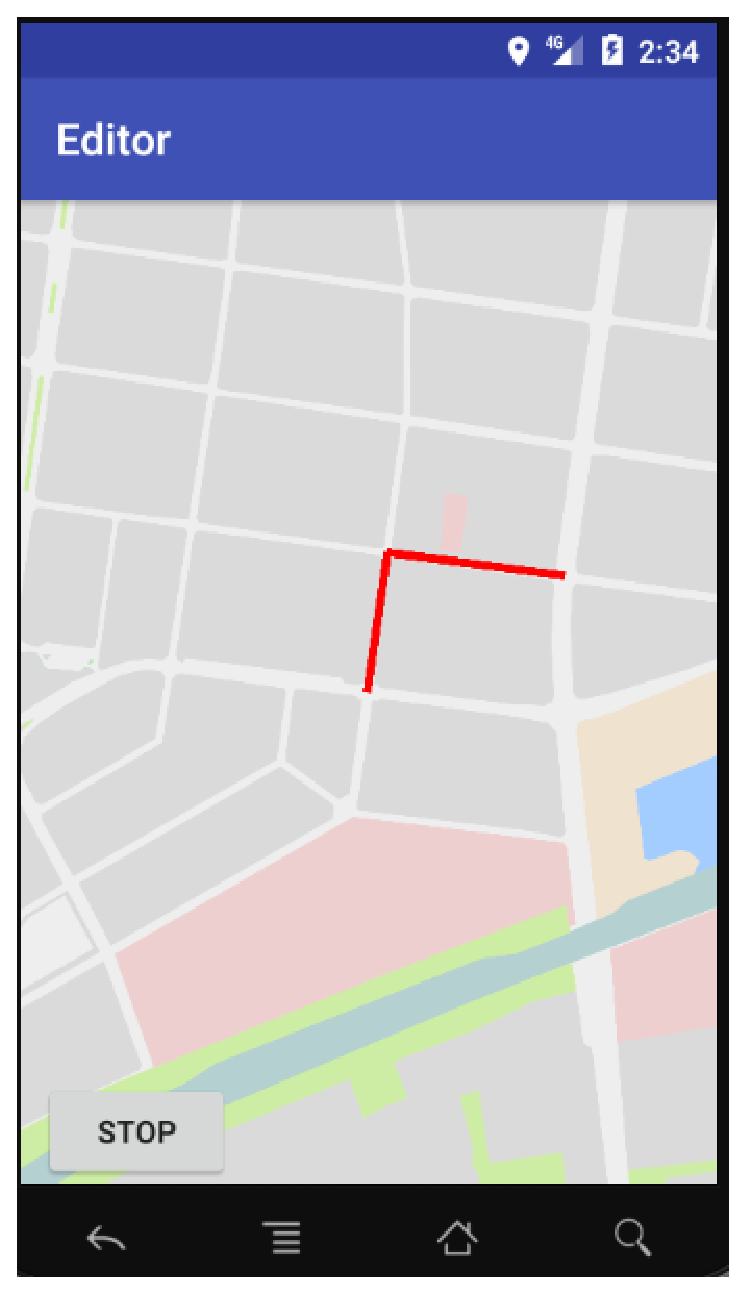
\includegraphics[width=0.7\textwidth]{AndroidEditorOV}

\section{Architektur}

\subsection{Überblick}
Grafik der Teile der Komponente (wichtig: Benennung aller Schnittstellen). 
Anwendung der Komponente nennen (Use Case).

Übliche Interaktionen durch Interaktionsdiagramme.

(Ausfüllen in Prototyp-Phase)

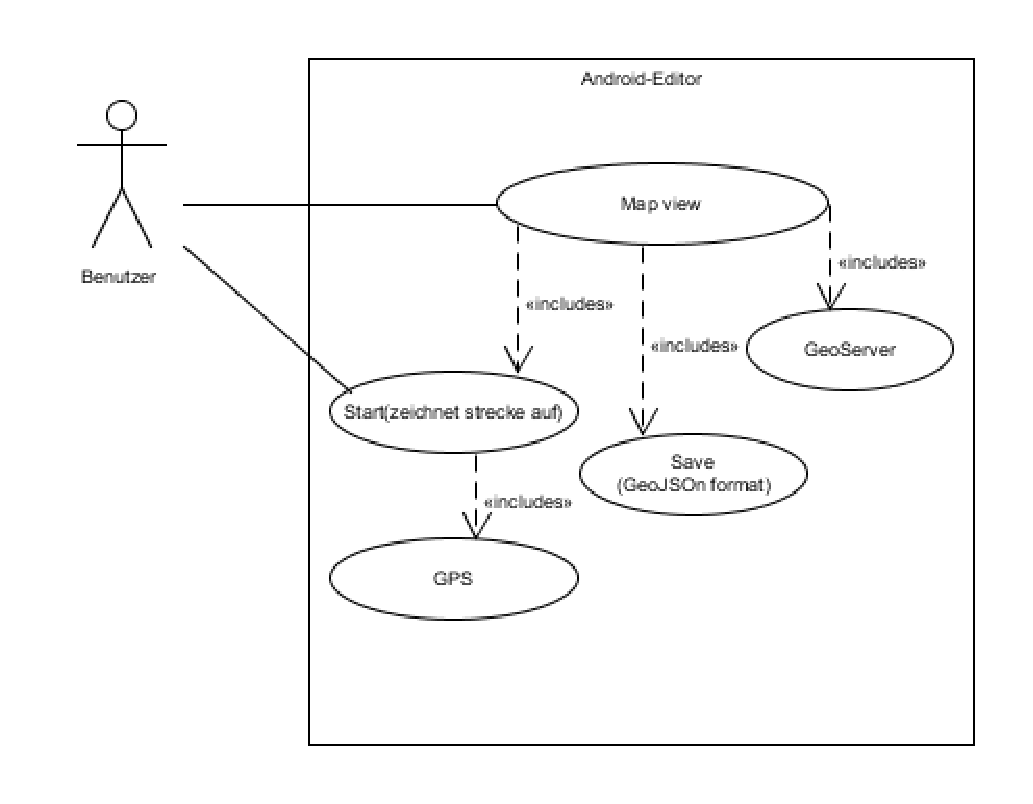
\includegraphics[width=1.0\textwidth]{UseCase}
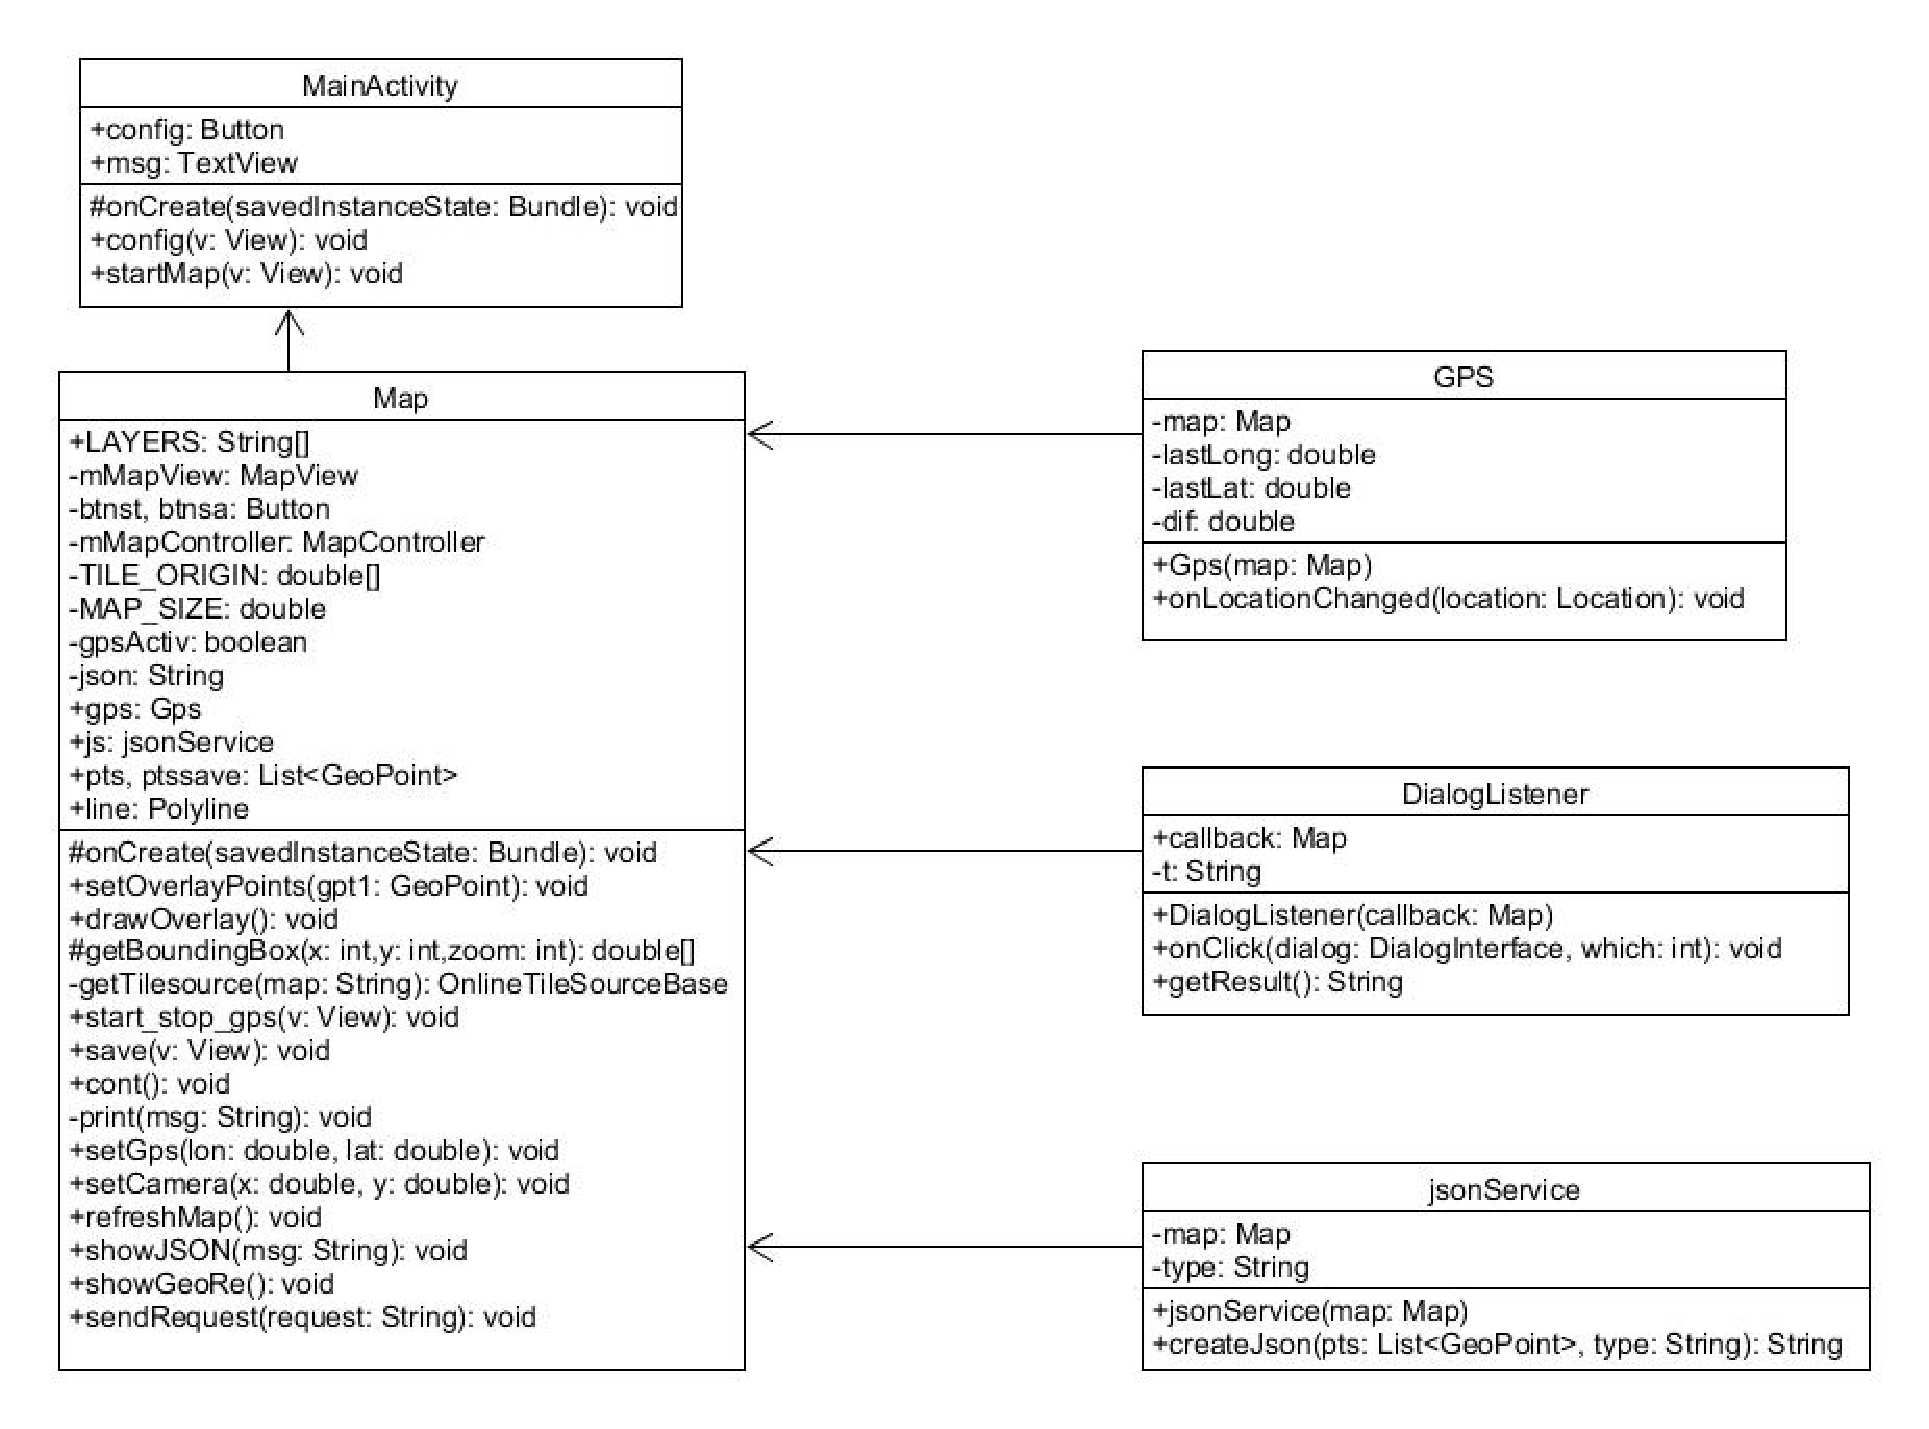
\includegraphics[width=0.7\textwidth]{OOA}

Der Editor bietet keine Schnittstellen nach außen. Jedoch soll die Import Schnittstelle verwendet werden um die Aufgezeichneten Daten der OHDM Datenbank hinzuzufügen.

Der Editor lädt sich die Layer, welche für die OHDM Map benötigt werden, von dem Geo-Server und erzeugt mithilfe der OSMdroid-Api eine Karte auf dem Smartphone. Der Nutzer hat die Möglichkeit eine Strecke oder ein Gebiet aufzuzeichnen und abzuspeichern. Des weiteren soll ein Zeitstempel und ein Name angegeben werden können um Historische Orte zu dokumentieren.

Die aufgezeichnete Strecke wird auf der Karte als Rote Linie Dargestellt, welche sich kontinuierlich während der aufzeichnungs-Phase verändert. Der Nutzer hat anschließend die Möglichkeit anzugeben um was es sich handelt (Gebiet,Punkt,Strecke). Die aufgezeichneten Daten werden als GeoJSON zwischengespeichert und sollen anschließend an die Import-Schnittelle übertragen werden.

\subsection{Schnittstellendefinitionen}

Diese Anwendung bietet keine Schnittstellen nach außen.

\subsection{genutztes Komponenten}
Beschreibung, welche weiteren Komponenten (in welchen Versionen, wo beziehbar) genutzt werden.

(Beginnen in Prototyp-Phase. Konkretisieren in der Alphaphase)

Momentan wird die OSMdroid-Api verwendet um die OHDM-Karte darzustellen.
Die App soll in einer Späteren Version die Import-Schnittstelle verwenden um die aufgezeichneten Daten(Koordinaten) zu übertragen.

\begin{table}[h]
 \begin{tabular}{|l|l|p{4cm}|}
 \hline
 API & Komponente & Kurzbeschreibung \\
 \hline
osmdroid & OnlineTileSourceBase & Dient dem generieren der URL, um Layer vom WMS-Server zu laden \newline 
 \\
 \hline
osmdroid & GeoPoint & Datenformat für Punkte(Koordinaten) \newline 
 \\
 \hline
osmdroid & MapController & dient dem verändern von Werten auf welche die MapView zurückgreift \newline 
 \\
 \hline
osmdroid & MapView & Darstellung der Karte \newline 
 \\
 \hline
osmdroid & Polyline & Dient zur Darstellung einer Linie auf der Karte \newline 
 \\
 \hline
 \end{tabular}
 \caption{Methodenbeschreibung}
 \end{table}


\section{Nutzung}
\subsection{Code}
Der Code befindet sich auf GitHub. \url{https://github.com/OpenHistoricalDataMap/OHDMAndroidEditor/}
Die verwendete IDE ist Android Studio.

\subsection{Deployment / Runtime}
Mittels der IDE Android Studio kann die App in einem Emulator gestartet oder direkt auf ein Device installiert werden.

\section{Qualitätssicherung}

App ist noch Sehr fehleranfällig, stürzte häufig ab, seit dem der stacked Layer eingefügt wurde stürzt die app kaum noch ab. Der Editor ist Momentan noch ein Prototyp.
Großteil der Fehler die Auftreten können werden abgefangen.

\subsection{Test}
Wie wird die Komponente getestet.

Getestet wir die Software durch manuell simulierte GPS Daten, und durch real abgelaufene strecken.

\section{Vorschläge / Ausblick}
Was ist aufgefallen, was sollte man ändern? Löschen Sie auch gern die Kommentare
der Vorgänger, aber nur, wenn es wirklich nicht mehr relevant ist.

Anfänglich gab es Probleme mit dem Laden der Layer. Die Ladezeit hatte für ein Gebiet fast 5 Minuten gedauert und es kam zu vielen Exceptions. Die Exceptions traten auf da für einige Koordinaten keine Layerdaten/Bilddaten existierten(vermutlich zu genaue Koordinaten). Durch den StackedLayer(Multilayer) wurde dieses Problem gelöst. Die Ladezeit ist nun annehmbar(ca 1 Minute) und es treten kaum bis keine Exceptions mehr auf.

Die aufgezeichneten Strecken sind sehr genau und es treten viele kleine Abweichungen auf. Aus diesem Grund wurde wurde eine Abweichungsbegrenzung von 1 Meter gesetzt. Alle Koordinaten welche eine Abweichung von weniger als 1 Meter von den vorher aufgezeichneten Koordinaten haben werden ignoriert und nicht aufgezeichnet.

Bisher ist noch nicht die Import-Schnittstelle eingebunden, das heißt die Daten werden bisher nicht in der Datenbank aufgenommen, jedoch schon ins GeoJSON-Format umgewandelt und testweise auf dem Display mit ausgegeben.

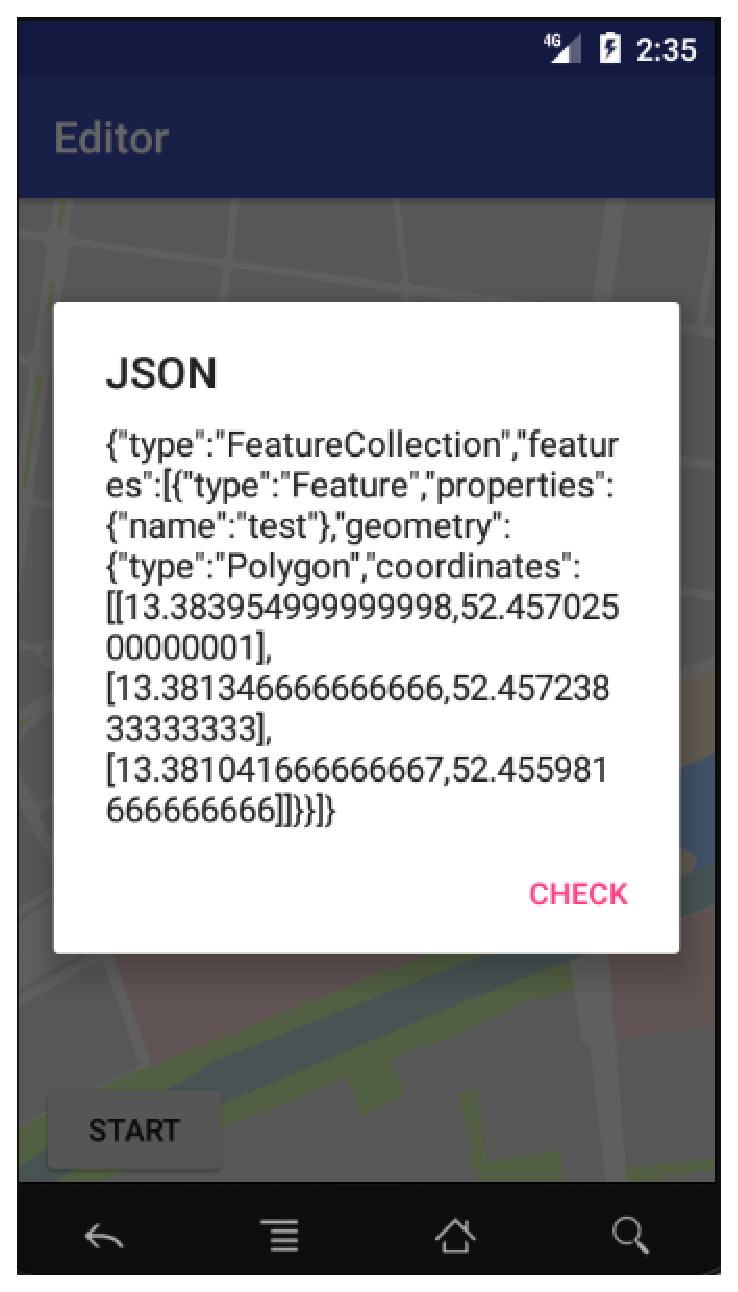
\includegraphics[width=0.7\textwidth]{AndroidEditorJSON}

\chapter{Linked Data Schnittstelle}
\graphicspath{ {img/} }

\section{Dokumentengeschichte}
\begin{table}[h]
 \begin{tabular}{|l|l|p{4cm}|}
 \hline
 Zeitraum & PL/Autor(en) & Änderungen \\
 \hline
 Wintersemester 2017/2018 & Georg Grauberger & 
Aufgabe der Komponente \newline
Architektur \newline
genutzte Komponenten
 \\
 \hline
 Wintersemester 1980/81 & IHR NAME & 
 \\
 \hline
 \end{tabular}
 \caption{Dokumentengeschichte}
 \end{table}

\section{Aufgabe der Komponente}
Die Aufgabe der Linked Data Schnittstelle ist es die OHDM Datenbank ueber
eine REST Schnittstelle im WWW verfuegbar zu machen.\newline
Die Daten sollen dann aufeinander verweisen so das man durch diese navigieren
kann. Die Objekte die durch die Schnittstelle freigegeben werden sind Geoobjekte
im geoJson Format.
\section{Architektur}

\subsection{Überlick}
Grafik der Teile der Komponente (wichtig: Benennung aller Schnittstellen). 
Anwendung der Komponente nennen (Use Case).

Übliche Interaktionen durch Interaktionsdiagramme.

Eine Spezifische Architektur fuer diese Komponente gibt es nicht, da wir die Richtlinien
des Spring-Boot Frameworks verwenden.
Als grobe zusammenfassung kann man jedoch sagen das das spring-boot das MVC Muster verwendet.
Wir implementieren also mit unserem Code die Model Schicht indem wir ein Mapping
fuer die Tabellen erstellen.
Die View und der Controller werden von dem maven Plugin 'spring-boot-starter' erstellt.
Das passiert automatisch da 'spring-boot' im Sinne von CoC agiert.

\subsection{Schnittstellendefinitionen}
Beschreibung der angebotenen Schnittstellen. Benennung der Funktionen
mit Vor- und Nachbedingungen. Beschreibuung des Protocol-Bindings.

(Beginnen in Prototyp-Phase. Konkretisieren in der Alphaphase)

\subsection{genutzte Komponenten}

\begin{table}[h]
\begin{tabular}{|l|p{4cm}|}
   \hline 
   Komponente & Beschreibung \\
   \hline
   \href{https://docs.spring.io/spring-data/jpa/docs/current/reference/html/}{spring-boot-data-jpa} &
    Ist verantwortlich fuer die Datenschicht, gibt Zugriff auf die Java Persistence API
   \\ \hline
   \href{https://docs.spring.io/spring-data/rest/docs/current/reference/html/}{spring-boot-starter-data-rest} &
   Beinhaltet viele automatismen um schnell eine REST Schnittstelle zu schaffen.
   \\ \hline
   \href{https://docs.spring.io/spring-data/rest/docs/current/reference/html/#_the_hal_browser}{spring-data-rest-hal-browser} &
   Beinhaltet einen REST Api browser mit dem man die Schnittstelle testen kann.
   \\ \hline
   \href{https://docs.spring.io/spring-boot/docs/current/reference/htmlsingle/#using-boot-starter}{spring-boot-starter-tomcat} &
   Beinhaltet einen Tomcat Server so das man zum Lokalen Testen und Starten keine einzelstehende Instanz
   vom Tomcat braucht.
   \\ \hline
   \href{https://docs.spring.io/spring-boot/docs/current/reference/html/using-boot-devtools.html}{spring-boot-devtools} &
   Beinhaltet Konfiguration fuer Quickreload und Quickdeployment in der Entwicklungsumgebung.
   \\ \hline
   postgresql &
   Beinhaltet den JDBC Treiber fuer PostGres.
   \\ \hline
\end{tabular}
\end{table}
\section{Nutzung}
\subsection{Code}
Den Code der Schnittstelle kann man auf GitHub über den Link finden: \\
\url{https://github.com/OpenHistoricalDataMap/LOD} \\
\\
Für die Realisierung der Schnittstelle wurde MVC-Framework Spring-Boot 
verwendet, dadurch hat der Code folgende Struktur: \\
\\
\includegraphics[scale=0.7]{image} \\
\\
\\
Alle notwendige Einstellungen für die Verbindung mit dem GeoServer sind 
in der Datei \textbf{application.properties} zu finden.
Modelle und deren Repositorien liegen entsprechend in Verzeichnissen 
\textbf{model} und \textbf{repository}. \\
\\
\\
\\
Struktur von \textbf{application.properties}:

\lstset{frame=single,basicstyle=\ttfamily\footnotesize,breaklines=true}

\begin{lstlisting}
# Datenquelle
spring.datasource.url = jdbc:[Driver]://[Host]:[Port]/[Datenbank]
spring.datasource.username = [Benutzername]
spring.datasource.password = [Passwort]

# Datenbank beim Startup initializieren
spring.jpa.hibernate.ddl-auto = [none|validate|update|create|create-drop]

spring.jpa.properties.hibernate.dialect = [Dialekt]
spring.jpa.properties.hibernate.default_schema = [DefaultSchema]
\end{lstlisting}
\vspace{5mm}
\noindent
Beispielhafte Einstellungen in \textbf{application.properties}:

\begin{lstlisting}
spring.datasource.url = jdbc:postgresql://htw.de:8000/test
spring.datasource.username = mustermann
spring.datasource.password = admin1234

spring.jpa.hibernate.ddl-auto = none
spring.jpa.properties.hibernate.dialect = org.hibernate.dialect.PostgreSQL9Dialect
spring.jpa.properties.hibernate.default_schema = ohdm
\end{lstlisting}

\subsection{Deployment / Runtime}
Das LOD-Server kann lokal durch die Kommandozeile mit folgenden Befehle aus 
dem Root-Verzeichnis des Projektes gestartet werden:\\
\\
Windows (mit cmd.exe):
\begin{lstlisting}
mvnw.cmd spring-boot:run
\end{lstlisting}
Linux und macOS:
\begin{lstlisting}
mvn spring-boot:run
\end{lstlisting}
Das lokale Server wird dann über die URL \textbf{127.0.0.1:8080} 
(oder localhost:8080) verfügbar.\\
\\
Um die Anwendung auf ein Webserver zu installieren, muss man zuerst eine WAR-Datei 
(Web Application Resource) erzeugen. Dafur stehen folgene Befehle zur Verfügung: \\
\\
Windows (mit cmd.exe):
\begin{lstlisting}
mvnw.cmd package
\end{lstlisting}
\vspace{10mm}
\noindent
Linux und macOS:
\begin{lstlisting}
mvn package
\end{lstlisting}
\vspace{5mm}
\noindent
Nach dem Ausführen des Befehls wird eine WAR-Datei im Ordner \textbf{target} 
des Root-Verzeichnises erstellt. Diese Datei kann dann auf ein Tomcat-Webserver
hochgeladen und ausgeführt werden.


\section{Qualitätssicherung}
(Ausfüllen ab Alpha-Phase).

Wie erfolgt die Sicherung der Qualität? Keine Romane, sondern ehrlich notieren,
was man tut. Wenn man nichts tut, dann steht hier: Wir sichern die Qualität der
Komponente nicht.

Issue-Tracking: wie erfolgt das, interne Fehlermeldungen (ab Alpha), 
externe Fehlermeldungen ab Beta.

\subsection{Test}
Wie wird die Komponente getestet.

\section{Vorschläge / Ausblick}
Was ist aufgefallen, was sollte man ändern? Löschen Sie auch gern die Kommentare
der Vorgänger, aber nur, wenn es wirklich nicht mehr relevant ist.



\chapter{SPARQL Schnittstelle}
\section{Dokumentengeschichte}
\begin{table}[h]
 \begin{tabular}{|l|l|p{4cm}|}
 \hline
 Zeitraum & PL/Autor(en) & Änderungen \\
 \hline
 Wintersemester 2017/2018 & IHR NAME & 
text \newline 
text \newline 
text \newline 
text \newline 
text \newline 
text \newline 
 
  \\
 \hline
 \end{tabular}
 \caption{Dokumentengeschichte}
 \end{table}

\section{Aufgabe der Komponente}

Server

Der Fuseki-Server verwaltet RDF-Dateien. Diese können in .rdf Format oder in .owl Formal in datasets hochgeladen werden.
In den datasets kann man auf die Triples in den Tabellen mit querys zugreifen. Ausgabe der Tabellen in JSON, XML, CSV und TSV als Raw Response. Raw Response auch zum direkt runterladen verfügbar. Die datasets auf den die Triples gelagert sind, kann man auch selbst erstellen unter "manage datasets" - > "add new dataset". Nach Bedarf "In-memory" oder "Persistens".


Verbale kurze prägnante Beschreibung, was die Komponente leisten soll.
Das sind wenige Seiten.

(Ausfüllen in Prototyp-Phase)

\section{Architektur}

\subsection{Überlick}
Grafik der Teile der Komponente (wichtig: Benennung aller Schnittstellen). 
Anwendung der Komponente nennen (Use Case).

Übliche Interaktionen durch Interaktionsdiagramme.

(Ausfüllen in Prototyp-Phase)

\subsection{Schnittstellendefinitionen}
Beschreibung der angebotenen Schnittstellen. Benennung der Funktionen
mit Vor- und Nachbedingungen. Beschreibuung des Protocol-Bindings.

(Beginnen in Prototyp-Phase. Konkretisieren in der Alphaphase)

\subsection{genutztes Komponenten}

Server

Den Server kann man direkt auf der Homepage jena.apache.org runterladen (aktuelle Version 3.6.0).
Nach dem entpacken muss man den "fuseki-server" mit chmod die Ausführrechte geben.
Anschließend kann man dann mit ./fuseki-server den Server zum laufen bringen.
Der Server läuft dann standartmäßig auf dem Port 3030 (Portfreigabe erforderlich).
Andere Ports möglich mit "./fuseki-server --port=*number*".

Im Verzeichnis run/ in der Datei shiro.ini kann man die Rechte vergeben.
Standart User, die nicht erstellt werden müssen, sind "anon" und "localhostFilter".
Um die Rechte für jeden Nutzer zu setzen muss man "anon" bearbeiten.
Um lokal die Rechte zu vergeben bearbeitet man "localhostFilter".
Zusätzlich kann man unter "[users]" eigene Nutzer mit Passwort setzen, den man dann auch Rechte vergeben.

Beschreibung, welche weiteren Komponenten (in welchen Versionen, wo beziehbar) genutzt werden.

(Beginnen in Prototyp-Phase. Konkretisieren in der Alphaphase)

\section{Nutzung}
\subsection{Code}
Wo findet man den Code. Struktur des Codes. (In Prototyphase ausfüllen,
kann dort sehr kurz sein. Ab Alpha-Phase konkret beschreiben.)

\subsection{Deployment / Runtime}
Beschreibung wie die Komponenten aus dem Quellcode erzeugt werden kann,
wie sie installiert wird und wie man sie startet.

\section{Qualitätssicherung}
(Ausfüllen ab Alpha-Phase).

Wie erfolgt die Sicherung der Qualität? Keine Romane, sondern ehrlich notieren,
was man tut. Wenn man nichts tut, dann steht hier: Wir sichern die Qualität der
Komponente nicht.

Issue-Tracking: wie erfolgt das, interne Fehlermeldungen (ab Alpha), 
externe Fehlermeldungen ab Beta.

\subsection{Test}
Wie wird die Komponente getestet.

\section{Vorschläge / Ausblick}
Was ist aufgefallen, was sollte man ändern? Löschen Sie auch gern die Kommentare
der Vorgänger, aber nur, wenn es wirklich nicht mehr relevant ist.



\chapter{GeoSPARQL Schnittstelle}
\section{Dokumentengeschichte}
\begin{table}[h]
 \begin{tabular}{|l|l|p{4cm}|}
 \hline
 Zeitraum & PL/Autor(en) & Änderungen \\
 \hline
 Sommersemester 2017 & Schulz, Daniel & 
Kapitel erstellt und Software dokumentiert \newline  
  \\
 \hline
 \end{tabular}
 \caption{Dokumentengeschichte}
 \end{table}

\section{Aufgabe der Komponente}

Bei den OHDM OfflineMaps (oder auch der OHDMApp) mit Xamarin handelt es sich um eine mobile Anwendung, welche vorab einen Datenexport aus OHDM erhält und danach in der Lage ist auf dem mobilen Gerät offline die entsprechenden Karten zu einem selbst bestimmbaren Zeitpunkt zu rendern.
So kann in der App beispielsweise der 01.02.1790 ausgewählt werden und es würden die zu diesem Datum gültigen Kartendaten dargestellt werden.
Da die Anwendung auf Xamarin und C\# basiert kann sie jederzeit mit geringem Aufwand auch auf iOS portiert und ausgerollt werden. (Bisher wird nur Android unterstützt)

\section{Architektur}

\subsection{Überlick}\label{ch:offlineoverview}

\hspace*{-3em}
\includegraphics*[width=1.3\linewidth,natwidth=1137,natheight=1042]{offlinemaps/bilder/komponentendiagramm.png}

In der obenstehenden durch Visual Studio automatisiert generierten CodeMap lassen sich die einzelnen Bestandteile der Xamarin-Anwendung ablesen, sowie die extern eingebundenen Bibliotheken/NuGet-Pakete.\\
\newpage
Nachfolgend werden alle Bestandteile sehr kurz erläutert:\\
\\
\begin{itemize}
	\item MainActivity: Diese Klasse ist für das UserInterface unter Android zuständig und definiert jegliche Interaktion mit dem Benutzer.
	\item MapDrawer: Diese Klasse definiert die grundlegende Darstellung von Kartenelementen, also zum Beispiel in welchen Zoomstufen sie gerendert werden und welche Styles sie nutzen.
	\item CsvUtils: Diese Klasse beinhaltet die Implementierung der Übertragung der Kartendaten aus einer CSV, welche zuvor aus der OHDM-Datenbank erzeugt wurde in eine neue interne SQLite-Datenbank für die Anwendung.
	\item MapEventHandler, MapEventArgs, CsvEventHandler, CsvEventArgs: Diese Klassen definieren Events, welche bei den verschiedenen Datenverarbeitungsschritten der App genutzt werden um dem Anwender den Fortschritt zu signalisieren.
	\item Styles: In dieser Klasse werden die Styles definiert, welche der MapDrawer später anwendet. Dies sind zum Beispiel die Farbe und Stärke von Linien, Punkten oder Polygonen.
	\item DatabaseHelper: Der DatabaseHelper definiert die Schnittstellen und Funktionen zur Anbindung an die lokale SQLite-Datenbank, welche zur Datenhaltung der eingelesenen Kartendaten genutzt wird.
	\item PostgisObjectMap: Diese Klasse wird genutzt um die Felder der PostgisObjects auf die Spalten der Daten-CSV zu mappen.
	\item PostgisObject, PostgisPoint, PostgisPolygon, PostgisLine: Diese Klassen stellen die objektbasierte Darstellung der Daten aus der OHDM-Datenbank dar, welche vom Programm genutzt wird.
	\item GlobalData: Diese Klasse ist nur eine statische Klasse zur Zwischenspeicherung von Daten auf welche von mehreren Klassen zugegriffen werden muss von denen nicht alle den nötigen Kontext aufweisen.
\end{itemize}
\newpage
Nachfolgend werden alle externen Libraries erläutert, welche nicht automatisiert von Xamarin geladen oder benötigt werden, sondern spezifisch für die Anwendung erforderlich sind:\\
\\
\begin{itemize}
	\item CartoMobileSDK: Hierbei handelt es sich um das Karten-Framework Carto, welches zur Darstellung der Offline-Karten genutzt wird.\\ \url{https://carto.com/docs/carto-engine/mobile-sdk/}
	\item CsvHelper: Bei CsvHelper handelt es sich um ein .NET basiertes Framework zum automatisierten einlesen und mappen von Objekten aus einer CSV-Datei.\\
	\url{https://github.com/JoshClose/CsvHelper}
	\item Newtonsoft.JSON: Hierbei handelt es sich um ein Framework zur Serialisierung und Deserialisierung von Objekten in JSON-Objekte.\\
	\url{https://www.newtonsoft.com/json}
	\item SQLite-net: Hierbei handelt es sich um eine Multiplattform-Bibliothek, welche die Erzeugung und Anbindung von SQLite-Datenbanken ermöglicht.\\
	\url{https://github.com/praeclarum/sqlite-net}
\end{itemize}

\subsection{Schnittstellendefinitionen}\label{ch:offlineinterfaces}
Die einzige Quasi-Schnittstelle, welche von den OfflineMaps genutzt bzw. benötigt wird ist ein Datenexport mit OHDM-Daten aus einer OHDM-Datenbank.
Zum Einlesen wird ein CSV-File in der folgenden Struktur benötigt:\\
\begin{lstlisting}[
basicstyle=\footnotesize
]
id;name;type_target;classification_id;classname;subclassname;valid_since;
valid_until;point;line;polygon
19;"S Tiergarten";1;396;"public_transport";"stop_position";"2015-12-22";
"2017-07-10";"{""type"":""Point"",""coordinates"":[13.3364598,52.5142085]}";"";""
20;"S Tiergarten";1;542;"railway";"station";"2015-12-22";
"2017-07-10";"{""type"":""Point"",""coordinates"":[13.3364598,52.5142085]}";"";""
65;"Jakob-Kaiser-Platz";1;589;"highway";"motorway_junction";"2017-01-01";
"2017-07-10";"{""type"":""Point"",""coordinates"":[13.2906741,52.533132]}";"";""
112;"S Pichelsberg";1;542;"railway";"station";"2016-03-04";
"2017-07-10";"{""type"":""Point"",""coordinates"":[13.2275633,52.5102387]}";"";""
136;"S Schoeneberg";1;583;"highway";"bus_stop";"2016-03-11";
"2017-07-10";"{""type"":""Point"",""coordinates"":[13.3529104,52.4797246]}";"";""
\end{lstlisting}
\newpage
Aus der Berliner-OHDM-Datenbank, welche auf dem PostgreSQL-Server der HTW Berlin liegt können die Daten in diesem Format mit der folgenden Abfrage extrahiert werden:

\begin{lstlisting}[
basicstyle=\footnotesize
]
SELECT gog.id, go.name, gog.type_target, gog.classification_id, 
c.class as classname, c.subclassname, gog.valid_since, gog.valid_until, 
ST_AsGeoJSON(p.point) as point, ST_AsGeoJSON(l.line) as line, 
ST_AsGeoJSON(poly.polygon) as polygon

FROM berlin.geoobject as go, berlin.classification as c, berlin.geoobject_geometry as gog

LEFT OUTER JOIN berlin.points as p ON gog.type_target=1 AND gog.id_target=p.id

LEFT OUTER JOIN berlin.lines as l ON gog.type_target=2 AND gog.id_target=l.id

LEFT OUTER JOIN berlin.polygons as poly ON gog.type_target=3 AND gog.id_target=poly.id

WHERE go.id=gog.id_geoobject_source AND gog.classification_id=c.id AND 
gog.type_target>0 AND gog.type_target<4 AND 
(point IS NOT NULL OR line IS NOT NULL OR polygon IS NOT NULL);
\end{lstlisting}

Alternativ könnten die Daten auch aus den Rendering-Tabellen bezogen werden, hierzu müsste nur eine neue Abfrage entwickelt werden und das Programm von WGS84, welches bisher genutzt wird, auf Pseudo-Mercator umgestellt werden.

\subsection{Genutzte Komponenten}

In der Anwendung wurden die folgenden Komponenten, welche zuvor in Kapitel \ref{ch:offlineoverview} detaillierter beschrieben wurden in den angegebenen Versionen benutzt:\\
\\
\begin{itemize}
	\item CartoMobileSDK: Version 4.1.0
	\item CsvHelper: Version 2.16.3.0\\(Achtung! Diese Version ist wichtig, da in der nachfolgenden Version die Nutzung komplett umgestellt wurde und ein komplettes Rewrite des CSV-Codes erfordern würde.)
	\item Newtonsoft.JSON: Version 10.0.3
	\item SQLite-net bzw. sqlite-net-pcl: Version 1.4.118 
\end{itemize}
Alle Versionen können ganz normal über den in Visual Studio integrierten NuGet-Paketmanager installiert werden.
\newpage
\section{Nutzung}
\subsection{Code}
Der aktuelle Code kann unter\\ \url{https://github.com/OpenHistoricalDataMap/OfflineMaps}\\ bezogen werden. Die Struktur des Codes wurde bereits in Kapitel \ref{ch:offlineoverview} erläutert und grafisch dargestellt.

\subsection{Deployment / Runtime}
Als Vorbedingung für das Deployment müssen zuerst folgende Dinge auf dem PC, welcher eingesetzt werden soll vorliegen bzw. installiert sein:\\
\\\\
Android ADB-Treiber von dem Mobilgerät, auf welchem später die Anwendung deployed werden soll.\\
Der Standard-Google-Treiber kann hier bezogen werden:\\ \url{https://developer.android.com/studio/run/win-usb.html}\\
Alternativ sind noch diese möglich: \url{https://adb.clockworkmod.com}\\
Hierbei ist zu beachten, dass jeder Gerätehersteller zum Teil eigene Treiber benötigt, vor allem Samsung, diese sind separat im Internet zu beziehen.\\\\
Zusätzlich muss das USB-Debugging auf Android aktiviert werden, wie hier beschrieben:\\
\url{https://www.howtogeek.com/129728/how-to-access-the-developer-options-menu-and-enable-usb-debugging-on-android-4.2/}\\\\\\
Es muss ein Datenextrakt aus der OHDM-Datenbank in Form einer CSV-Datei vorliegen. In Kapitel \ref{ch:offlineinterfaces} wird erläutert, wie und in welchem Format dieser zu erzeugen ist.\\ Die Datei muss hinterher den Namen ``outputnew.csv'' erhalten.\\\\\\
Um das OfflineMaps-Projekt zu bearbeiten oder zu deployen ist als Entwicklungsumgebung Visual Studio 2017 mit Xamarin nötig.\\
Visual Studio 2017 kann theoretisch in der kostenlosen Community-Edition heruntergeladen und installiert werden, da aber für Hochschulangehöroge die Enterprise-Version über Microsoft Imagine/Dreamspark kostenlos bezogen werden kann, sollte diese genutzt werden und in der nachfolgenden Erläuterung wird auch nur auf diese eingegangen.\\
Informationen zum Download von Microsoft-Produkten für Hochschulangehörige der HTW Berlin finden sich hier:\\
\url{http://www.f4.htw-berlin.de/studieren/softwarelizenzen/}\\
Im nachfolgenden Link wird erläutert mit welchen Optionen Visual Studio 2017 installiert werden muss um Xamarin-Projekte zu unterstützen:\\
\url{https://developer.xamarin.com/guides/cross-platform/getting_started/installation/windows/}\\
Die Xamarin-Installation entsprechend dem Guide ist zwingend erforderlich!
Zusätzlich müssen im Installationsbildschirm von Visual Studio 2017, in welchem auch die Xamarin-Pakete angehakt werden auch zwingend alle Git und GitHub-Pakete, sowie Pakete, welche das Android SDK betreffen angehakt werden, hierzu sollten alle Unterpunkte durchgeklickt und durchsucht werden.\\\\
Nachdem Visual Studio 2017 mit allen zuvor beschriebenen Komponenten installiert wurde, kann es gestartet werden.\\
Anschließend kann man dem Tutorial von Microsoft zum Klonen eines Git-Repos ab dem Punkt ``Clone from another Git Provider'' folgen (die Punkte darüber können ignoriert werden):\\
\url{https://docs.microsoft.com/en-us/vsts/git/tutorial/clone?tabs=visual-studio#clone-from-another-git-provider}\\
Der Git-Link des Repos der OfflineMaps, welcher zum klonen eingesetzt wird lautet: 
\url{https://github.com/OpenHistoricalDataMap/OfflineMaps.git}\\
Gegebenfalls fragt VisualStudio vor dem Klonen noch die eigenen GitHub-Zugangsdaten ab.\\\\
Nachdem die Solution entsprechend der Angaben des Microsoft-Tutorials geklont und geöffnet wurde ist das Projekt nahezu bereit zum Deployment und es müssen nur noch zwei individuelle Schritte ausgeführt werden:\\\\
Zuerst muss in der AndroidManifest.xml, welche sich unter Properties befindet ein eigener Name für das Package gesetzt werden, da es sonst später zu Fehlern mit dem API-Key kommt.\\
In der Klasse MainActivity muss die Stringkonstante LICENSE in welcher nur exemplarisch ``XXX'' steht gegen einen eigenen API-Key von Carto ausgetauscht werden. Dieser kann von Carto kostenlos erzeugt werden gemäß der nachfolgenden Anleitung unter dem Punkt ``Registering your App'':\\
\url{https://carto.com/docs/carto-engine/mobile-sdk/getting-started/#registering-your-app}\\\\
Als letzten Schritt muss nur noch die im Projektverzeichnis unter Assets liegende ``outputnew.csv'' durch die ausgetauscht werden, welche gemäß Kapitel \ref{ch:offlineinterfaces} erzeugt wurde.\\\\
Danach kann die App durch einen Klick auf den grünen Pfeil im oberen Zentrum der Navigationsleisten oder einen Druck auf F5 auf dem (an den PC angeschlossenen) Android-Gerät deployed und ausgeführt werden.\\
Sollte es Fehlermeldungen wegen nicht korrekt geladener NuGet-Pakete geben, so können diese in der NuGet-Konsole (Extras -> NuGet-Paket-Manager -> Paket-Manager-Konsole) mit dem Befehl ``update-package -reinstall'' neu initialisiert werden.\\\\
Zusätzlicher Hinweis: Durch einen Bug im aktuellen Android-SDK verhält sich Android Oreo noch etwas seltsam, so schließt sich beim Ausführen über Visual Studio die Anwendung direkt wieder. Hier muss die Anwendung nachdem sie über Visual Studio installiert wurde einfach vom Handy aus gestartet werden, dann funktioniert alles. Für das Debugging sollte aus diesem Grund aktuell Android in der Version  $\leq7.1.2$ verwendet werden. Außerdem ist dringend anzuraten, alle Visual Studio und Android SDK Updates zu installieren.


\section{Qualitätssicherung}

Die Qualitätssicherung der Darstellung erfolgt bisher durch akribische Abgleiche der OHDM-Darstellung mit der aktuellen deutschen OSM-Darstellung und die Angleichung an dieselbe. Für das Handling der Anwendung was Verständlichkeit und Performance angeht wurde die Qualität durch externe unbeteiligte Personen bewertet und dann verbessert.\\
\\
Issue-Tracking: Bisher keines.

\subsection{Test}
Die Komponente kann momentan ausschließlich durch Anwender-Testgruppen getestet werden und nicht automatisiert, aufgrund der Komplexität der Darstellung. Es wäre allenfalls möglich die Datenimport und -Exportfunktionen um Unit-Tests zu erweitern, was aber aktuell noch nicht umgesetzt ist. 

\section{Vorschläge / Ausblick}
In der Anwendung sind bisher nur exemplarisch die wichtigsten Typen an OSM-Objekten mit spezifischen Rendering-Merkmalen für eine spezifische Darstellung versehen. Hier bietet es sich an auch die übrigen zu implementieren. Außerdem wäre es sinnvoll und gewinnbringend die vorhandene Xamarin-Codebasis zu erweitern und um die entsprechenden iOS und UWP-Schnittstellen zu erweitern um die Anwendung auch auf iOS- und Windows-Geräten zum Einsatz bringen zu können.

\chapter{Data Provenance}
\section{Dokumentengeschichte}
\begin{table}[h]
 \begin{tabular}{|l|l|p{4cm}|}
 \hline
 Zeitraum & PL/Autor(en) & Änderungen \\
 \hline
 Sommersemester 2017 & Schulz, Daniel & 
Kapitel erstellt und Software dokumentiert \newline  
  \\
 \hline
 \end{tabular}
 \caption{Dokumentengeschichte}
 \end{table}

\section{Aufgabe der Komponente}

Bei den OHDM OfflineMaps (oder auch der OHDMApp) mit Xamarin handelt es sich um eine mobile Anwendung, welche vorab einen Datenexport aus OHDM erhält und danach in der Lage ist auf dem mobilen Gerät offline die entsprechenden Karten zu einem selbst bestimmbaren Zeitpunkt zu rendern.
So kann in der App beispielsweise der 01.02.1790 ausgewählt werden und es würden die zu diesem Datum gültigen Kartendaten dargestellt werden.
Da die Anwendung auf Xamarin und C\# basiert kann sie jederzeit mit geringem Aufwand auch auf iOS portiert und ausgerollt werden. (Bisher wird nur Android unterstützt)

\section{Architektur}

\subsection{Überlick}\label{ch:offlineoverview}

\hspace*{-3em}
\includegraphics*[width=1.3\linewidth,natwidth=1137,natheight=1042]{offlinemaps/bilder/komponentendiagramm.png}

In der obenstehenden durch Visual Studio automatisiert generierten CodeMap lassen sich die einzelnen Bestandteile der Xamarin-Anwendung ablesen, sowie die extern eingebundenen Bibliotheken/NuGet-Pakete.\\
\newpage
Nachfolgend werden alle Bestandteile sehr kurz erläutert:\\
\\
\begin{itemize}
	\item MainActivity: Diese Klasse ist für das UserInterface unter Android zuständig und definiert jegliche Interaktion mit dem Benutzer.
	\item MapDrawer: Diese Klasse definiert die grundlegende Darstellung von Kartenelementen, also zum Beispiel in welchen Zoomstufen sie gerendert werden und welche Styles sie nutzen.
	\item CsvUtils: Diese Klasse beinhaltet die Implementierung der Übertragung der Kartendaten aus einer CSV, welche zuvor aus der OHDM-Datenbank erzeugt wurde in eine neue interne SQLite-Datenbank für die Anwendung.
	\item MapEventHandler, MapEventArgs, CsvEventHandler, CsvEventArgs: Diese Klassen definieren Events, welche bei den verschiedenen Datenverarbeitungsschritten der App genutzt werden um dem Anwender den Fortschritt zu signalisieren.
	\item Styles: In dieser Klasse werden die Styles definiert, welche der MapDrawer später anwendet. Dies sind zum Beispiel die Farbe und Stärke von Linien, Punkten oder Polygonen.
	\item DatabaseHelper: Der DatabaseHelper definiert die Schnittstellen und Funktionen zur Anbindung an die lokale SQLite-Datenbank, welche zur Datenhaltung der eingelesenen Kartendaten genutzt wird.
	\item PostgisObjectMap: Diese Klasse wird genutzt um die Felder der PostgisObjects auf die Spalten der Daten-CSV zu mappen.
	\item PostgisObject, PostgisPoint, PostgisPolygon, PostgisLine: Diese Klassen stellen die objektbasierte Darstellung der Daten aus der OHDM-Datenbank dar, welche vom Programm genutzt wird.
	\item GlobalData: Diese Klasse ist nur eine statische Klasse zur Zwischenspeicherung von Daten auf welche von mehreren Klassen zugegriffen werden muss von denen nicht alle den nötigen Kontext aufweisen.
\end{itemize}
\newpage
Nachfolgend werden alle externen Libraries erläutert, welche nicht automatisiert von Xamarin geladen oder benötigt werden, sondern spezifisch für die Anwendung erforderlich sind:\\
\\
\begin{itemize}
	\item CartoMobileSDK: Hierbei handelt es sich um das Karten-Framework Carto, welches zur Darstellung der Offline-Karten genutzt wird.\\ \url{https://carto.com/docs/carto-engine/mobile-sdk/}
	\item CsvHelper: Bei CsvHelper handelt es sich um ein .NET basiertes Framework zum automatisierten einlesen und mappen von Objekten aus einer CSV-Datei.\\
	\url{https://github.com/JoshClose/CsvHelper}
	\item Newtonsoft.JSON: Hierbei handelt es sich um ein Framework zur Serialisierung und Deserialisierung von Objekten in JSON-Objekte.\\
	\url{https://www.newtonsoft.com/json}
	\item SQLite-net: Hierbei handelt es sich um eine Multiplattform-Bibliothek, welche die Erzeugung und Anbindung von SQLite-Datenbanken ermöglicht.\\
	\url{https://github.com/praeclarum/sqlite-net}
\end{itemize}

\subsection{Schnittstellendefinitionen}\label{ch:offlineinterfaces}
Die einzige Quasi-Schnittstelle, welche von den OfflineMaps genutzt bzw. benötigt wird ist ein Datenexport mit OHDM-Daten aus einer OHDM-Datenbank.
Zum Einlesen wird ein CSV-File in der folgenden Struktur benötigt:\\
\begin{lstlisting}[
basicstyle=\footnotesize
]
id;name;type_target;classification_id;classname;subclassname;valid_since;
valid_until;point;line;polygon
19;"S Tiergarten";1;396;"public_transport";"stop_position";"2015-12-22";
"2017-07-10";"{""type"":""Point"",""coordinates"":[13.3364598,52.5142085]}";"";""
20;"S Tiergarten";1;542;"railway";"station";"2015-12-22";
"2017-07-10";"{""type"":""Point"",""coordinates"":[13.3364598,52.5142085]}";"";""
65;"Jakob-Kaiser-Platz";1;589;"highway";"motorway_junction";"2017-01-01";
"2017-07-10";"{""type"":""Point"",""coordinates"":[13.2906741,52.533132]}";"";""
112;"S Pichelsberg";1;542;"railway";"station";"2016-03-04";
"2017-07-10";"{""type"":""Point"",""coordinates"":[13.2275633,52.5102387]}";"";""
136;"S Schoeneberg";1;583;"highway";"bus_stop";"2016-03-11";
"2017-07-10";"{""type"":""Point"",""coordinates"":[13.3529104,52.4797246]}";"";""
\end{lstlisting}
\newpage
Aus der Berliner-OHDM-Datenbank, welche auf dem PostgreSQL-Server der HTW Berlin liegt können die Daten in diesem Format mit der folgenden Abfrage extrahiert werden:

\begin{lstlisting}[
basicstyle=\footnotesize
]
SELECT gog.id, go.name, gog.type_target, gog.classification_id, 
c.class as classname, c.subclassname, gog.valid_since, gog.valid_until, 
ST_AsGeoJSON(p.point) as point, ST_AsGeoJSON(l.line) as line, 
ST_AsGeoJSON(poly.polygon) as polygon

FROM berlin.geoobject as go, berlin.classification as c, berlin.geoobject_geometry as gog

LEFT OUTER JOIN berlin.points as p ON gog.type_target=1 AND gog.id_target=p.id

LEFT OUTER JOIN berlin.lines as l ON gog.type_target=2 AND gog.id_target=l.id

LEFT OUTER JOIN berlin.polygons as poly ON gog.type_target=3 AND gog.id_target=poly.id

WHERE go.id=gog.id_geoobject_source AND gog.classification_id=c.id AND 
gog.type_target>0 AND gog.type_target<4 AND 
(point IS NOT NULL OR line IS NOT NULL OR polygon IS NOT NULL);
\end{lstlisting}

Alternativ könnten die Daten auch aus den Rendering-Tabellen bezogen werden, hierzu müsste nur eine neue Abfrage entwickelt werden und das Programm von WGS84, welches bisher genutzt wird, auf Pseudo-Mercator umgestellt werden.

\subsection{Genutzte Komponenten}

In der Anwendung wurden die folgenden Komponenten, welche zuvor in Kapitel \ref{ch:offlineoverview} detaillierter beschrieben wurden in den angegebenen Versionen benutzt:\\
\\
\begin{itemize}
	\item CartoMobileSDK: Version 4.1.0
	\item CsvHelper: Version 2.16.3.0\\(Achtung! Diese Version ist wichtig, da in der nachfolgenden Version die Nutzung komplett umgestellt wurde und ein komplettes Rewrite des CSV-Codes erfordern würde.)
	\item Newtonsoft.JSON: Version 10.0.3
	\item SQLite-net bzw. sqlite-net-pcl: Version 1.4.118 
\end{itemize}
Alle Versionen können ganz normal über den in Visual Studio integrierten NuGet-Paketmanager installiert werden.
\newpage
\section{Nutzung}
\subsection{Code}
Der aktuelle Code kann unter\\ \url{https://github.com/OpenHistoricalDataMap/OfflineMaps}\\ bezogen werden. Die Struktur des Codes wurde bereits in Kapitel \ref{ch:offlineoverview} erläutert und grafisch dargestellt.

\subsection{Deployment / Runtime}
Als Vorbedingung für das Deployment müssen zuerst folgende Dinge auf dem PC, welcher eingesetzt werden soll vorliegen bzw. installiert sein:\\
\\\\
Android ADB-Treiber von dem Mobilgerät, auf welchem später die Anwendung deployed werden soll.\\
Der Standard-Google-Treiber kann hier bezogen werden:\\ \url{https://developer.android.com/studio/run/win-usb.html}\\
Alternativ sind noch diese möglich: \url{https://adb.clockworkmod.com}\\
Hierbei ist zu beachten, dass jeder Gerätehersteller zum Teil eigene Treiber benötigt, vor allem Samsung, diese sind separat im Internet zu beziehen.\\\\
Zusätzlich muss das USB-Debugging auf Android aktiviert werden, wie hier beschrieben:\\
\url{https://www.howtogeek.com/129728/how-to-access-the-developer-options-menu-and-enable-usb-debugging-on-android-4.2/}\\\\\\
Es muss ein Datenextrakt aus der OHDM-Datenbank in Form einer CSV-Datei vorliegen. In Kapitel \ref{ch:offlineinterfaces} wird erläutert, wie und in welchem Format dieser zu erzeugen ist.\\ Die Datei muss hinterher den Namen ``outputnew.csv'' erhalten.\\\\\\
Um das OfflineMaps-Projekt zu bearbeiten oder zu deployen ist als Entwicklungsumgebung Visual Studio 2017 mit Xamarin nötig.\\
Visual Studio 2017 kann theoretisch in der kostenlosen Community-Edition heruntergeladen und installiert werden, da aber für Hochschulangehöroge die Enterprise-Version über Microsoft Imagine/Dreamspark kostenlos bezogen werden kann, sollte diese genutzt werden und in der nachfolgenden Erläuterung wird auch nur auf diese eingegangen.\\
Informationen zum Download von Microsoft-Produkten für Hochschulangehörige der HTW Berlin finden sich hier:\\
\url{http://www.f4.htw-berlin.de/studieren/softwarelizenzen/}\\
Im nachfolgenden Link wird erläutert mit welchen Optionen Visual Studio 2017 installiert werden muss um Xamarin-Projekte zu unterstützen:\\
\url{https://developer.xamarin.com/guides/cross-platform/getting_started/installation/windows/}\\
Die Xamarin-Installation entsprechend dem Guide ist zwingend erforderlich!
Zusätzlich müssen im Installationsbildschirm von Visual Studio 2017, in welchem auch die Xamarin-Pakete angehakt werden auch zwingend alle Git und GitHub-Pakete, sowie Pakete, welche das Android SDK betreffen angehakt werden, hierzu sollten alle Unterpunkte durchgeklickt und durchsucht werden.\\\\
Nachdem Visual Studio 2017 mit allen zuvor beschriebenen Komponenten installiert wurde, kann es gestartet werden.\\
Anschließend kann man dem Tutorial von Microsoft zum Klonen eines Git-Repos ab dem Punkt ``Clone from another Git Provider'' folgen (die Punkte darüber können ignoriert werden):\\
\url{https://docs.microsoft.com/en-us/vsts/git/tutorial/clone?tabs=visual-studio#clone-from-another-git-provider}\\
Der Git-Link des Repos der OfflineMaps, welcher zum klonen eingesetzt wird lautet: 
\url{https://github.com/OpenHistoricalDataMap/OfflineMaps.git}\\
Gegebenfalls fragt VisualStudio vor dem Klonen noch die eigenen GitHub-Zugangsdaten ab.\\\\
Nachdem die Solution entsprechend der Angaben des Microsoft-Tutorials geklont und geöffnet wurde ist das Projekt nahezu bereit zum Deployment und es müssen nur noch zwei individuelle Schritte ausgeführt werden:\\\\
Zuerst muss in der AndroidManifest.xml, welche sich unter Properties befindet ein eigener Name für das Package gesetzt werden, da es sonst später zu Fehlern mit dem API-Key kommt.\\
In der Klasse MainActivity muss die Stringkonstante LICENSE in welcher nur exemplarisch ``XXX'' steht gegen einen eigenen API-Key von Carto ausgetauscht werden. Dieser kann von Carto kostenlos erzeugt werden gemäß der nachfolgenden Anleitung unter dem Punkt ``Registering your App'':\\
\url{https://carto.com/docs/carto-engine/mobile-sdk/getting-started/#registering-your-app}\\\\
Als letzten Schritt muss nur noch die im Projektverzeichnis unter Assets liegende ``outputnew.csv'' durch die ausgetauscht werden, welche gemäß Kapitel \ref{ch:offlineinterfaces} erzeugt wurde.\\\\
Danach kann die App durch einen Klick auf den grünen Pfeil im oberen Zentrum der Navigationsleisten oder einen Druck auf F5 auf dem (an den PC angeschlossenen) Android-Gerät deployed und ausgeführt werden.\\
Sollte es Fehlermeldungen wegen nicht korrekt geladener NuGet-Pakete geben, so können diese in der NuGet-Konsole (Extras -> NuGet-Paket-Manager -> Paket-Manager-Konsole) mit dem Befehl ``update-package -reinstall'' neu initialisiert werden.\\\\
Zusätzlicher Hinweis: Durch einen Bug im aktuellen Android-SDK verhält sich Android Oreo noch etwas seltsam, so schließt sich beim Ausführen über Visual Studio die Anwendung direkt wieder. Hier muss die Anwendung nachdem sie über Visual Studio installiert wurde einfach vom Handy aus gestartet werden, dann funktioniert alles. Für das Debugging sollte aus diesem Grund aktuell Android in der Version  $\leq7.1.2$ verwendet werden. Außerdem ist dringend anzuraten, alle Visual Studio und Android SDK Updates zu installieren.


\section{Qualitätssicherung}

Die Qualitätssicherung der Darstellung erfolgt bisher durch akribische Abgleiche der OHDM-Darstellung mit der aktuellen deutschen OSM-Darstellung und die Angleichung an dieselbe. Für das Handling der Anwendung was Verständlichkeit und Performance angeht wurde die Qualität durch externe unbeteiligte Personen bewertet und dann verbessert.\\
\\
Issue-Tracking: Bisher keines.

\subsection{Test}
Die Komponente kann momentan ausschließlich durch Anwender-Testgruppen getestet werden und nicht automatisiert, aufgrund der Komplexität der Darstellung. Es wäre allenfalls möglich die Datenimport und -Exportfunktionen um Unit-Tests zu erweitern, was aber aktuell noch nicht umgesetzt ist. 

\section{Vorschläge / Ausblick}
In der Anwendung sind bisher nur exemplarisch die wichtigsten Typen an OSM-Objekten mit spezifischen Rendering-Merkmalen für eine spezifische Darstellung versehen. Hier bietet es sich an auch die übrigen zu implementieren. Außerdem wäre es sinnvoll und gewinnbringend die vorhandene Xamarin-Codebasis zu erweitern und um die entsprechenden iOS und UWP-Schnittstellen zu erweitern um die Anwendung auch auf iOS- und Windows-Geräten zum Einsatz bringen zu können.

\chapter{CIDOC CRM Unterstützung}
\section{Dokumentengeschichte}
\begin{table}[h]
 \begin{tabular}{|l|l|p{4cm}|}
 \hline
 Zeitraum & PL/Autor(en) & Änderungen \\
 \hline
 Sommersemester 2017 & Schulz, Daniel & 
Kapitel erstellt und Software dokumentiert \newline  
  \\
 \hline
 \end{tabular}
 \caption{Dokumentengeschichte}
 \end{table}

\section{Aufgabe der Komponente}

Bei den OHDM OfflineMaps (oder auch der OHDMApp) mit Xamarin handelt es sich um eine mobile Anwendung, welche vorab einen Datenexport aus OHDM erhält und danach in der Lage ist auf dem mobilen Gerät offline die entsprechenden Karten zu einem selbst bestimmbaren Zeitpunkt zu rendern.
So kann in der App beispielsweise der 01.02.1790 ausgewählt werden und es würden die zu diesem Datum gültigen Kartendaten dargestellt werden.
Da die Anwendung auf Xamarin und C\# basiert kann sie jederzeit mit geringem Aufwand auch auf iOS portiert und ausgerollt werden. (Bisher wird nur Android unterstützt)

\section{Architektur}

\subsection{Überlick}\label{ch:offlineoverview}

\hspace*{-3em}
\includegraphics*[width=1.3\linewidth,natwidth=1137,natheight=1042]{offlinemaps/bilder/komponentendiagramm.png}

In der obenstehenden durch Visual Studio automatisiert generierten CodeMap lassen sich die einzelnen Bestandteile der Xamarin-Anwendung ablesen, sowie die extern eingebundenen Bibliotheken/NuGet-Pakete.\\
\newpage
Nachfolgend werden alle Bestandteile sehr kurz erläutert:\\
\\
\begin{itemize}
	\item MainActivity: Diese Klasse ist für das UserInterface unter Android zuständig und definiert jegliche Interaktion mit dem Benutzer.
	\item MapDrawer: Diese Klasse definiert die grundlegende Darstellung von Kartenelementen, also zum Beispiel in welchen Zoomstufen sie gerendert werden und welche Styles sie nutzen.
	\item CsvUtils: Diese Klasse beinhaltet die Implementierung der Übertragung der Kartendaten aus einer CSV, welche zuvor aus der OHDM-Datenbank erzeugt wurde in eine neue interne SQLite-Datenbank für die Anwendung.
	\item MapEventHandler, MapEventArgs, CsvEventHandler, CsvEventArgs: Diese Klassen definieren Events, welche bei den verschiedenen Datenverarbeitungsschritten der App genutzt werden um dem Anwender den Fortschritt zu signalisieren.
	\item Styles: In dieser Klasse werden die Styles definiert, welche der MapDrawer später anwendet. Dies sind zum Beispiel die Farbe und Stärke von Linien, Punkten oder Polygonen.
	\item DatabaseHelper: Der DatabaseHelper definiert die Schnittstellen und Funktionen zur Anbindung an die lokale SQLite-Datenbank, welche zur Datenhaltung der eingelesenen Kartendaten genutzt wird.
	\item PostgisObjectMap: Diese Klasse wird genutzt um die Felder der PostgisObjects auf die Spalten der Daten-CSV zu mappen.
	\item PostgisObject, PostgisPoint, PostgisPolygon, PostgisLine: Diese Klassen stellen die objektbasierte Darstellung der Daten aus der OHDM-Datenbank dar, welche vom Programm genutzt wird.
	\item GlobalData: Diese Klasse ist nur eine statische Klasse zur Zwischenspeicherung von Daten auf welche von mehreren Klassen zugegriffen werden muss von denen nicht alle den nötigen Kontext aufweisen.
\end{itemize}
\newpage
Nachfolgend werden alle externen Libraries erläutert, welche nicht automatisiert von Xamarin geladen oder benötigt werden, sondern spezifisch für die Anwendung erforderlich sind:\\
\\
\begin{itemize}
	\item CartoMobileSDK: Hierbei handelt es sich um das Karten-Framework Carto, welches zur Darstellung der Offline-Karten genutzt wird.\\ \url{https://carto.com/docs/carto-engine/mobile-sdk/}
	\item CsvHelper: Bei CsvHelper handelt es sich um ein .NET basiertes Framework zum automatisierten einlesen und mappen von Objekten aus einer CSV-Datei.\\
	\url{https://github.com/JoshClose/CsvHelper}
	\item Newtonsoft.JSON: Hierbei handelt es sich um ein Framework zur Serialisierung und Deserialisierung von Objekten in JSON-Objekte.\\
	\url{https://www.newtonsoft.com/json}
	\item SQLite-net: Hierbei handelt es sich um eine Multiplattform-Bibliothek, welche die Erzeugung und Anbindung von SQLite-Datenbanken ermöglicht.\\
	\url{https://github.com/praeclarum/sqlite-net}
\end{itemize}

\subsection{Schnittstellendefinitionen}\label{ch:offlineinterfaces}
Die einzige Quasi-Schnittstelle, welche von den OfflineMaps genutzt bzw. benötigt wird ist ein Datenexport mit OHDM-Daten aus einer OHDM-Datenbank.
Zum Einlesen wird ein CSV-File in der folgenden Struktur benötigt:\\
\begin{lstlisting}[
basicstyle=\footnotesize
]
id;name;type_target;classification_id;classname;subclassname;valid_since;
valid_until;point;line;polygon
19;"S Tiergarten";1;396;"public_transport";"stop_position";"2015-12-22";
"2017-07-10";"{""type"":""Point"",""coordinates"":[13.3364598,52.5142085]}";"";""
20;"S Tiergarten";1;542;"railway";"station";"2015-12-22";
"2017-07-10";"{""type"":""Point"",""coordinates"":[13.3364598,52.5142085]}";"";""
65;"Jakob-Kaiser-Platz";1;589;"highway";"motorway_junction";"2017-01-01";
"2017-07-10";"{""type"":""Point"",""coordinates"":[13.2906741,52.533132]}";"";""
112;"S Pichelsberg";1;542;"railway";"station";"2016-03-04";
"2017-07-10";"{""type"":""Point"",""coordinates"":[13.2275633,52.5102387]}";"";""
136;"S Schoeneberg";1;583;"highway";"bus_stop";"2016-03-11";
"2017-07-10";"{""type"":""Point"",""coordinates"":[13.3529104,52.4797246]}";"";""
\end{lstlisting}
\newpage
Aus der Berliner-OHDM-Datenbank, welche auf dem PostgreSQL-Server der HTW Berlin liegt können die Daten in diesem Format mit der folgenden Abfrage extrahiert werden:

\begin{lstlisting}[
basicstyle=\footnotesize
]
SELECT gog.id, go.name, gog.type_target, gog.classification_id, 
c.class as classname, c.subclassname, gog.valid_since, gog.valid_until, 
ST_AsGeoJSON(p.point) as point, ST_AsGeoJSON(l.line) as line, 
ST_AsGeoJSON(poly.polygon) as polygon

FROM berlin.geoobject as go, berlin.classification as c, berlin.geoobject_geometry as gog

LEFT OUTER JOIN berlin.points as p ON gog.type_target=1 AND gog.id_target=p.id

LEFT OUTER JOIN berlin.lines as l ON gog.type_target=2 AND gog.id_target=l.id

LEFT OUTER JOIN berlin.polygons as poly ON gog.type_target=3 AND gog.id_target=poly.id

WHERE go.id=gog.id_geoobject_source AND gog.classification_id=c.id AND 
gog.type_target>0 AND gog.type_target<4 AND 
(point IS NOT NULL OR line IS NOT NULL OR polygon IS NOT NULL);
\end{lstlisting}

Alternativ könnten die Daten auch aus den Rendering-Tabellen bezogen werden, hierzu müsste nur eine neue Abfrage entwickelt werden und das Programm von WGS84, welches bisher genutzt wird, auf Pseudo-Mercator umgestellt werden.

\subsection{Genutzte Komponenten}

In der Anwendung wurden die folgenden Komponenten, welche zuvor in Kapitel \ref{ch:offlineoverview} detaillierter beschrieben wurden in den angegebenen Versionen benutzt:\\
\\
\begin{itemize}
	\item CartoMobileSDK: Version 4.1.0
	\item CsvHelper: Version 2.16.3.0\\(Achtung! Diese Version ist wichtig, da in der nachfolgenden Version die Nutzung komplett umgestellt wurde und ein komplettes Rewrite des CSV-Codes erfordern würde.)
	\item Newtonsoft.JSON: Version 10.0.3
	\item SQLite-net bzw. sqlite-net-pcl: Version 1.4.118 
\end{itemize}
Alle Versionen können ganz normal über den in Visual Studio integrierten NuGet-Paketmanager installiert werden.
\newpage
\section{Nutzung}
\subsection{Code}
Der aktuelle Code kann unter\\ \url{https://github.com/OpenHistoricalDataMap/OfflineMaps}\\ bezogen werden. Die Struktur des Codes wurde bereits in Kapitel \ref{ch:offlineoverview} erläutert und grafisch dargestellt.

\subsection{Deployment / Runtime}
Als Vorbedingung für das Deployment müssen zuerst folgende Dinge auf dem PC, welcher eingesetzt werden soll vorliegen bzw. installiert sein:\\
\\\\
Android ADB-Treiber von dem Mobilgerät, auf welchem später die Anwendung deployed werden soll.\\
Der Standard-Google-Treiber kann hier bezogen werden:\\ \url{https://developer.android.com/studio/run/win-usb.html}\\
Alternativ sind noch diese möglich: \url{https://adb.clockworkmod.com}\\
Hierbei ist zu beachten, dass jeder Gerätehersteller zum Teil eigene Treiber benötigt, vor allem Samsung, diese sind separat im Internet zu beziehen.\\\\
Zusätzlich muss das USB-Debugging auf Android aktiviert werden, wie hier beschrieben:\\
\url{https://www.howtogeek.com/129728/how-to-access-the-developer-options-menu-and-enable-usb-debugging-on-android-4.2/}\\\\\\
Es muss ein Datenextrakt aus der OHDM-Datenbank in Form einer CSV-Datei vorliegen. In Kapitel \ref{ch:offlineinterfaces} wird erläutert, wie und in welchem Format dieser zu erzeugen ist.\\ Die Datei muss hinterher den Namen ``outputnew.csv'' erhalten.\\\\\\
Um das OfflineMaps-Projekt zu bearbeiten oder zu deployen ist als Entwicklungsumgebung Visual Studio 2017 mit Xamarin nötig.\\
Visual Studio 2017 kann theoretisch in der kostenlosen Community-Edition heruntergeladen und installiert werden, da aber für Hochschulangehöroge die Enterprise-Version über Microsoft Imagine/Dreamspark kostenlos bezogen werden kann, sollte diese genutzt werden und in der nachfolgenden Erläuterung wird auch nur auf diese eingegangen.\\
Informationen zum Download von Microsoft-Produkten für Hochschulangehörige der HTW Berlin finden sich hier:\\
\url{http://www.f4.htw-berlin.de/studieren/softwarelizenzen/}\\
Im nachfolgenden Link wird erläutert mit welchen Optionen Visual Studio 2017 installiert werden muss um Xamarin-Projekte zu unterstützen:\\
\url{https://developer.xamarin.com/guides/cross-platform/getting_started/installation/windows/}\\
Die Xamarin-Installation entsprechend dem Guide ist zwingend erforderlich!
Zusätzlich müssen im Installationsbildschirm von Visual Studio 2017, in welchem auch die Xamarin-Pakete angehakt werden auch zwingend alle Git und GitHub-Pakete, sowie Pakete, welche das Android SDK betreffen angehakt werden, hierzu sollten alle Unterpunkte durchgeklickt und durchsucht werden.\\\\
Nachdem Visual Studio 2017 mit allen zuvor beschriebenen Komponenten installiert wurde, kann es gestartet werden.\\
Anschließend kann man dem Tutorial von Microsoft zum Klonen eines Git-Repos ab dem Punkt ``Clone from another Git Provider'' folgen (die Punkte darüber können ignoriert werden):\\
\url{https://docs.microsoft.com/en-us/vsts/git/tutorial/clone?tabs=visual-studio#clone-from-another-git-provider}\\
Der Git-Link des Repos der OfflineMaps, welcher zum klonen eingesetzt wird lautet: 
\url{https://github.com/OpenHistoricalDataMap/OfflineMaps.git}\\
Gegebenfalls fragt VisualStudio vor dem Klonen noch die eigenen GitHub-Zugangsdaten ab.\\\\
Nachdem die Solution entsprechend der Angaben des Microsoft-Tutorials geklont und geöffnet wurde ist das Projekt nahezu bereit zum Deployment und es müssen nur noch zwei individuelle Schritte ausgeführt werden:\\\\
Zuerst muss in der AndroidManifest.xml, welche sich unter Properties befindet ein eigener Name für das Package gesetzt werden, da es sonst später zu Fehlern mit dem API-Key kommt.\\
In der Klasse MainActivity muss die Stringkonstante LICENSE in welcher nur exemplarisch ``XXX'' steht gegen einen eigenen API-Key von Carto ausgetauscht werden. Dieser kann von Carto kostenlos erzeugt werden gemäß der nachfolgenden Anleitung unter dem Punkt ``Registering your App'':\\
\url{https://carto.com/docs/carto-engine/mobile-sdk/getting-started/#registering-your-app}\\\\
Als letzten Schritt muss nur noch die im Projektverzeichnis unter Assets liegende ``outputnew.csv'' durch die ausgetauscht werden, welche gemäß Kapitel \ref{ch:offlineinterfaces} erzeugt wurde.\\\\
Danach kann die App durch einen Klick auf den grünen Pfeil im oberen Zentrum der Navigationsleisten oder einen Druck auf F5 auf dem (an den PC angeschlossenen) Android-Gerät deployed und ausgeführt werden.\\
Sollte es Fehlermeldungen wegen nicht korrekt geladener NuGet-Pakete geben, so können diese in der NuGet-Konsole (Extras -> NuGet-Paket-Manager -> Paket-Manager-Konsole) mit dem Befehl ``update-package -reinstall'' neu initialisiert werden.\\\\
Zusätzlicher Hinweis: Durch einen Bug im aktuellen Android-SDK verhält sich Android Oreo noch etwas seltsam, so schließt sich beim Ausführen über Visual Studio die Anwendung direkt wieder. Hier muss die Anwendung nachdem sie über Visual Studio installiert wurde einfach vom Handy aus gestartet werden, dann funktioniert alles. Für das Debugging sollte aus diesem Grund aktuell Android in der Version  $\leq7.1.2$ verwendet werden. Außerdem ist dringend anzuraten, alle Visual Studio und Android SDK Updates zu installieren.


\section{Qualitätssicherung}

Die Qualitätssicherung der Darstellung erfolgt bisher durch akribische Abgleiche der OHDM-Darstellung mit der aktuellen deutschen OSM-Darstellung und die Angleichung an dieselbe. Für das Handling der Anwendung was Verständlichkeit und Performance angeht wurde die Qualität durch externe unbeteiligte Personen bewertet und dann verbessert.\\
\\
Issue-Tracking: Bisher keines.

\subsection{Test}
Die Komponente kann momentan ausschließlich durch Anwender-Testgruppen getestet werden und nicht automatisiert, aufgrund der Komplexität der Darstellung. Es wäre allenfalls möglich die Datenimport und -Exportfunktionen um Unit-Tests zu erweitern, was aber aktuell noch nicht umgesetzt ist. 

\section{Vorschläge / Ausblick}
In der Anwendung sind bisher nur exemplarisch die wichtigsten Typen an OSM-Objekten mit spezifischen Rendering-Merkmalen für eine spezifische Darstellung versehen. Hier bietet es sich an auch die übrigen zu implementieren. Außerdem wäre es sinnvoll und gewinnbringend die vorhandene Xamarin-Codebasis zu erweitern und um die entsprechenden iOS und UWP-Schnittstellen zu erweitern um die Anwendung auch auf iOS- und Windows-Geräten zum Einsatz bringen zu können.

\chapter{OHDM OfflineMaps mit Xamarin}
\section{Dokumentengeschichte}
\begin{table}[h]
 \begin{tabular}{|l|l|p{4cm}|}
 \hline
 Zeitraum & PL/Autor(en) & Änderungen \\
 \hline
 Sommersemester 2017 & Schulz, Daniel & 
Kapitel erstellt und Software dokumentiert \newline  
  \\
 \hline
 \end{tabular}
 \caption{Dokumentengeschichte}
 \end{table}

\section{Aufgabe der Komponente}

Bei den OHDM OfflineMaps (oder auch der OHDMApp) mit Xamarin handelt es sich um eine mobile Anwendung, welche vorab einen Datenexport aus OHDM erhält und danach in der Lage ist auf dem mobilen Gerät offline die entsprechenden Karten zu einem selbst bestimmbaren Zeitpunkt zu rendern.
So kann in der App beispielsweise der 01.02.1790 ausgewählt werden und es würden die zu diesem Datum gültigen Kartendaten dargestellt werden.
Da die Anwendung auf Xamarin und C\# basiert kann sie jederzeit mit geringem Aufwand auch auf iOS portiert und ausgerollt werden. (Bisher wird nur Android unterstützt)

\section{Architektur}

\subsection{Überlick}\label{ch:offlineoverview}

\hspace*{-3em}
\includegraphics*[width=1.3\linewidth,natwidth=1137,natheight=1042]{offlinemaps/bilder/komponentendiagramm.png}

In der obenstehenden durch Visual Studio automatisiert generierten CodeMap lassen sich die einzelnen Bestandteile der Xamarin-Anwendung ablesen, sowie die extern eingebundenen Bibliotheken/NuGet-Pakete.\\
\newpage
Nachfolgend werden alle Bestandteile sehr kurz erläutert:\\
\\
\begin{itemize}
	\item MainActivity: Diese Klasse ist für das UserInterface unter Android zuständig und definiert jegliche Interaktion mit dem Benutzer.
	\item MapDrawer: Diese Klasse definiert die grundlegende Darstellung von Kartenelementen, also zum Beispiel in welchen Zoomstufen sie gerendert werden und welche Styles sie nutzen.
	\item CsvUtils: Diese Klasse beinhaltet die Implementierung der Übertragung der Kartendaten aus einer CSV, welche zuvor aus der OHDM-Datenbank erzeugt wurde in eine neue interne SQLite-Datenbank für die Anwendung.
	\item MapEventHandler, MapEventArgs, CsvEventHandler, CsvEventArgs: Diese Klassen definieren Events, welche bei den verschiedenen Datenverarbeitungsschritten der App genutzt werden um dem Anwender den Fortschritt zu signalisieren.
	\item Styles: In dieser Klasse werden die Styles definiert, welche der MapDrawer später anwendet. Dies sind zum Beispiel die Farbe und Stärke von Linien, Punkten oder Polygonen.
	\item DatabaseHelper: Der DatabaseHelper definiert die Schnittstellen und Funktionen zur Anbindung an die lokale SQLite-Datenbank, welche zur Datenhaltung der eingelesenen Kartendaten genutzt wird.
	\item PostgisObjectMap: Diese Klasse wird genutzt um die Felder der PostgisObjects auf die Spalten der Daten-CSV zu mappen.
	\item PostgisObject, PostgisPoint, PostgisPolygon, PostgisLine: Diese Klassen stellen die objektbasierte Darstellung der Daten aus der OHDM-Datenbank dar, welche vom Programm genutzt wird.
	\item GlobalData: Diese Klasse ist nur eine statische Klasse zur Zwischenspeicherung von Daten auf welche von mehreren Klassen zugegriffen werden muss von denen nicht alle den nötigen Kontext aufweisen.
\end{itemize}
\newpage
Nachfolgend werden alle externen Libraries erläutert, welche nicht automatisiert von Xamarin geladen oder benötigt werden, sondern spezifisch für die Anwendung erforderlich sind:\\
\\
\begin{itemize}
	\item CartoMobileSDK: Hierbei handelt es sich um das Karten-Framework Carto, welches zur Darstellung der Offline-Karten genutzt wird.\\ \url{https://carto.com/docs/carto-engine/mobile-sdk/}
	\item CsvHelper: Bei CsvHelper handelt es sich um ein .NET basiertes Framework zum automatisierten einlesen und mappen von Objekten aus einer CSV-Datei.\\
	\url{https://github.com/JoshClose/CsvHelper}
	\item Newtonsoft.JSON: Hierbei handelt es sich um ein Framework zur Serialisierung und Deserialisierung von Objekten in JSON-Objekte.\\
	\url{https://www.newtonsoft.com/json}
	\item SQLite-net: Hierbei handelt es sich um eine Multiplattform-Bibliothek, welche die Erzeugung und Anbindung von SQLite-Datenbanken ermöglicht.\\
	\url{https://github.com/praeclarum/sqlite-net}
\end{itemize}

\subsection{Schnittstellendefinitionen}\label{ch:offlineinterfaces}
Die einzige Quasi-Schnittstelle, welche von den OfflineMaps genutzt bzw. benötigt wird ist ein Datenexport mit OHDM-Daten aus einer OHDM-Datenbank.
Zum Einlesen wird ein CSV-File in der folgenden Struktur benötigt:\\
\begin{lstlisting}[
basicstyle=\footnotesize
]
id;name;type_target;classification_id;classname;subclassname;valid_since;
valid_until;point;line;polygon
19;"S Tiergarten";1;396;"public_transport";"stop_position";"2015-12-22";
"2017-07-10";"{""type"":""Point"",""coordinates"":[13.3364598,52.5142085]}";"";""
20;"S Tiergarten";1;542;"railway";"station";"2015-12-22";
"2017-07-10";"{""type"":""Point"",""coordinates"":[13.3364598,52.5142085]}";"";""
65;"Jakob-Kaiser-Platz";1;589;"highway";"motorway_junction";"2017-01-01";
"2017-07-10";"{""type"":""Point"",""coordinates"":[13.2906741,52.533132]}";"";""
112;"S Pichelsberg";1;542;"railway";"station";"2016-03-04";
"2017-07-10";"{""type"":""Point"",""coordinates"":[13.2275633,52.5102387]}";"";""
136;"S Schoeneberg";1;583;"highway";"bus_stop";"2016-03-11";
"2017-07-10";"{""type"":""Point"",""coordinates"":[13.3529104,52.4797246]}";"";""
\end{lstlisting}
\newpage
Aus der Berliner-OHDM-Datenbank, welche auf dem PostgreSQL-Server der HTW Berlin liegt können die Daten in diesem Format mit der folgenden Abfrage extrahiert werden:

\begin{lstlisting}[
basicstyle=\footnotesize
]
SELECT gog.id, go.name, gog.type_target, gog.classification_id, 
c.class as classname, c.subclassname, gog.valid_since, gog.valid_until, 
ST_AsGeoJSON(p.point) as point, ST_AsGeoJSON(l.line) as line, 
ST_AsGeoJSON(poly.polygon) as polygon

FROM berlin.geoobject as go, berlin.classification as c, berlin.geoobject_geometry as gog

LEFT OUTER JOIN berlin.points as p ON gog.type_target=1 AND gog.id_target=p.id

LEFT OUTER JOIN berlin.lines as l ON gog.type_target=2 AND gog.id_target=l.id

LEFT OUTER JOIN berlin.polygons as poly ON gog.type_target=3 AND gog.id_target=poly.id

WHERE go.id=gog.id_geoobject_source AND gog.classification_id=c.id AND 
gog.type_target>0 AND gog.type_target<4 AND 
(point IS NOT NULL OR line IS NOT NULL OR polygon IS NOT NULL);
\end{lstlisting}

Alternativ könnten die Daten auch aus den Rendering-Tabellen bezogen werden, hierzu müsste nur eine neue Abfrage entwickelt werden und das Programm von WGS84, welches bisher genutzt wird, auf Pseudo-Mercator umgestellt werden.

\subsection{Genutzte Komponenten}

In der Anwendung wurden die folgenden Komponenten, welche zuvor in Kapitel \ref{ch:offlineoverview} detaillierter beschrieben wurden in den angegebenen Versionen benutzt:\\
\\
\begin{itemize}
	\item CartoMobileSDK: Version 4.1.0
	\item CsvHelper: Version 2.16.3.0\\(Achtung! Diese Version ist wichtig, da in der nachfolgenden Version die Nutzung komplett umgestellt wurde und ein komplettes Rewrite des CSV-Codes erfordern würde.)
	\item Newtonsoft.JSON: Version 10.0.3
	\item SQLite-net bzw. sqlite-net-pcl: Version 1.4.118 
\end{itemize}
Alle Versionen können ganz normal über den in Visual Studio integrierten NuGet-Paketmanager installiert werden.
\newpage
\section{Nutzung}
\subsection{Code}
Der aktuelle Code kann unter\\ \url{https://github.com/OpenHistoricalDataMap/OfflineMaps}\\ bezogen werden. Die Struktur des Codes wurde bereits in Kapitel \ref{ch:offlineoverview} erläutert und grafisch dargestellt.

\subsection{Deployment / Runtime}
Als Vorbedingung für das Deployment müssen zuerst folgende Dinge auf dem PC, welcher eingesetzt werden soll vorliegen bzw. installiert sein:\\
\\\\
Android ADB-Treiber von dem Mobilgerät, auf welchem später die Anwendung deployed werden soll.\\
Der Standard-Google-Treiber kann hier bezogen werden:\\ \url{https://developer.android.com/studio/run/win-usb.html}\\
Alternativ sind noch diese möglich: \url{https://adb.clockworkmod.com}\\
Hierbei ist zu beachten, dass jeder Gerätehersteller zum Teil eigene Treiber benötigt, vor allem Samsung, diese sind separat im Internet zu beziehen.\\\\
Zusätzlich muss das USB-Debugging auf Android aktiviert werden, wie hier beschrieben:\\
\url{https://www.howtogeek.com/129728/how-to-access-the-developer-options-menu-and-enable-usb-debugging-on-android-4.2/}\\\\\\
Es muss ein Datenextrakt aus der OHDM-Datenbank in Form einer CSV-Datei vorliegen. In Kapitel \ref{ch:offlineinterfaces} wird erläutert, wie und in welchem Format dieser zu erzeugen ist.\\ Die Datei muss hinterher den Namen ``outputnew.csv'' erhalten.\\\\\\
Um das OfflineMaps-Projekt zu bearbeiten oder zu deployen ist als Entwicklungsumgebung Visual Studio 2017 mit Xamarin nötig.\\
Visual Studio 2017 kann theoretisch in der kostenlosen Community-Edition heruntergeladen und installiert werden, da aber für Hochschulangehöroge die Enterprise-Version über Microsoft Imagine/Dreamspark kostenlos bezogen werden kann, sollte diese genutzt werden und in der nachfolgenden Erläuterung wird auch nur auf diese eingegangen.\\
Informationen zum Download von Microsoft-Produkten für Hochschulangehörige der HTW Berlin finden sich hier:\\
\url{http://www.f4.htw-berlin.de/studieren/softwarelizenzen/}\\
Im nachfolgenden Link wird erläutert mit welchen Optionen Visual Studio 2017 installiert werden muss um Xamarin-Projekte zu unterstützen:\\
\url{https://developer.xamarin.com/guides/cross-platform/getting_started/installation/windows/}\\
Die Xamarin-Installation entsprechend dem Guide ist zwingend erforderlich!
Zusätzlich müssen im Installationsbildschirm von Visual Studio 2017, in welchem auch die Xamarin-Pakete angehakt werden auch zwingend alle Git und GitHub-Pakete, sowie Pakete, welche das Android SDK betreffen angehakt werden, hierzu sollten alle Unterpunkte durchgeklickt und durchsucht werden.\\\\
Nachdem Visual Studio 2017 mit allen zuvor beschriebenen Komponenten installiert wurde, kann es gestartet werden.\\
Anschließend kann man dem Tutorial von Microsoft zum Klonen eines Git-Repos ab dem Punkt ``Clone from another Git Provider'' folgen (die Punkte darüber können ignoriert werden):\\
\url{https://docs.microsoft.com/en-us/vsts/git/tutorial/clone?tabs=visual-studio#clone-from-another-git-provider}\\
Der Git-Link des Repos der OfflineMaps, welcher zum klonen eingesetzt wird lautet: 
\url{https://github.com/OpenHistoricalDataMap/OfflineMaps.git}\\
Gegebenfalls fragt VisualStudio vor dem Klonen noch die eigenen GitHub-Zugangsdaten ab.\\\\
Nachdem die Solution entsprechend der Angaben des Microsoft-Tutorials geklont und geöffnet wurde ist das Projekt nahezu bereit zum Deployment und es müssen nur noch zwei individuelle Schritte ausgeführt werden:\\\\
Zuerst muss in der AndroidManifest.xml, welche sich unter Properties befindet ein eigener Name für das Package gesetzt werden, da es sonst später zu Fehlern mit dem API-Key kommt.\\
In der Klasse MainActivity muss die Stringkonstante LICENSE in welcher nur exemplarisch ``XXX'' steht gegen einen eigenen API-Key von Carto ausgetauscht werden. Dieser kann von Carto kostenlos erzeugt werden gemäß der nachfolgenden Anleitung unter dem Punkt ``Registering your App'':\\
\url{https://carto.com/docs/carto-engine/mobile-sdk/getting-started/#registering-your-app}\\\\
Als letzten Schritt muss nur noch die im Projektverzeichnis unter Assets liegende ``outputnew.csv'' durch die ausgetauscht werden, welche gemäß Kapitel \ref{ch:offlineinterfaces} erzeugt wurde.\\\\
Danach kann die App durch einen Klick auf den grünen Pfeil im oberen Zentrum der Navigationsleisten oder einen Druck auf F5 auf dem (an den PC angeschlossenen) Android-Gerät deployed und ausgeführt werden.\\
Sollte es Fehlermeldungen wegen nicht korrekt geladener NuGet-Pakete geben, so können diese in der NuGet-Konsole (Extras -> NuGet-Paket-Manager -> Paket-Manager-Konsole) mit dem Befehl ``update-package -reinstall'' neu initialisiert werden.\\\\
Zusätzlicher Hinweis: Durch einen Bug im aktuellen Android-SDK verhält sich Android Oreo noch etwas seltsam, so schließt sich beim Ausführen über Visual Studio die Anwendung direkt wieder. Hier muss die Anwendung nachdem sie über Visual Studio installiert wurde einfach vom Handy aus gestartet werden, dann funktioniert alles. Für das Debugging sollte aus diesem Grund aktuell Android in der Version  $\leq7.1.2$ verwendet werden. Außerdem ist dringend anzuraten, alle Visual Studio und Android SDK Updates zu installieren.


\section{Qualitätssicherung}

Die Qualitätssicherung der Darstellung erfolgt bisher durch akribische Abgleiche der OHDM-Darstellung mit der aktuellen deutschen OSM-Darstellung und die Angleichung an dieselbe. Für das Handling der Anwendung was Verständlichkeit und Performance angeht wurde die Qualität durch externe unbeteiligte Personen bewertet und dann verbessert.\\
\\
Issue-Tracking: Bisher keines.

\subsection{Test}
Die Komponente kann momentan ausschließlich durch Anwender-Testgruppen getestet werden und nicht automatisiert, aufgrund der Komplexität der Darstellung. Es wäre allenfalls möglich die Datenimport und -Exportfunktionen um Unit-Tests zu erweitern, was aber aktuell noch nicht umgesetzt ist. 

\section{Vorschläge / Ausblick}
In der Anwendung sind bisher nur exemplarisch die wichtigsten Typen an OSM-Objekten mit spezifischen Rendering-Merkmalen für eine spezifische Darstellung versehen. Hier bietet es sich an auch die übrigen zu implementieren. Außerdem wäre es sinnvoll und gewinnbringend die vorhandene Xamarin-Codebasis zu erweitern und um die entsprechenden iOS und UWP-Schnittstellen zu erweitern um die Anwendung auch auf iOS- und Windows-Geräten zum Einsatz bringen zu können.

\end{document}
